\documentclass[sensors,article,submit,pdftex]{mdpi}

% ──────────────────────────────────────────────────────────────
% Math commands and theorem environments
% ──────────────────────────────────────────────────────────────
\newcommand{\vect}[1]{\boldsymbol{#1}}
\newcommand{\mat}[1]{\mathbf{#1}}
\newcommand{\R}{\mathbb{R}}
\newcommand{\E}{\mathbb{E}}
\newcommand{\Prob}{\mathbb{P}}
\DeclareMathOperator*{\argmin}{arg\,min}
\DeclareMathOperator*{\argmax}{arg\,max}
\DeclareMathOperator{\tr}{tr}
\DeclareMathOperator{\diag}{diag}

% Code listing style (if not using listings from class)
\lstdefinestyle{algo}{
    basicstyle=\footnotesize\ttfamily,
    frame=single, numbers=left, numberstyle=\tiny, numbersep=5pt,
    xleftmargin=15pt, framexleftmargin=15pt, breaklines=true, columns=flexible,
}

\begin{document}

% ══════════════════════════════════════════════════════
% TITLE AND AUTHOR INFORMATION
% ══════════════════════════════════════════════════════
\Title{AeroGraphRX: Simulation of a Graph Signal Processing Framework for Real-Time RF Signal Detection and Flight Tracking}

\Author{Usha A\textsuperscript{1}, Noel George\textsuperscript{1,*}}

\address{\textsuperscript{1}Department of Pure and Applied Mathematics, Alliance School of Applied Mathematics, Alliance University, Bengaluru 562106, India}

\corres{\textsuperscript{*}Corresponding author: \href{mailto:gnoelPDF25@sam.alliance.edu.in}{gnoelPDF25@sam.alliance.edu.in}}

\maketitle

% ══════════════════════════════════════════════════════
% ABSTRACT AND KEYWORDS
% ══════════════════════════════════════════════════════
\begin{MDPIabstract}
Modern signal intelligence (SIGINT) and electronic surveillance systems require the convergence of massive radio frequency (RF) data ingestion, adaptive detection algorithms, and rigorous evaluation. This paper presents a simulation study of \textbf{AeroGraphRX}, a hybrid open-source architecture integrating: (i)~OpenWebRX as the distributed software-defined radio (SDR) data-collection front end; (ii)~graph theory and graph signal processing (GSP) for modelling temporal, spatial, and spectral relationships via the graph Laplacian $\mat{L} = \mat{D} - \mat{W}$ and graph Fourier transform; and (iii)~receiver operating characteristic (ROC) analysis for threshold-independent classifier evaluation. The framework is evaluated through comprehensive Monte Carlo simulation across four core capabilities: real-time flight tracking via time-difference-of-arrival (TDoA) multilateration with joint probabilistic data association (JPDA); convolutional--graph convolutional network (CNN-GCN) hybrid signal classification; stealth aircraft detection through graph anomaly scoring with analytically derived false alarm control; and unknown signal identification---including extra-terrestrial technosignature candidates---using variational autoencoders (VAE). Monte Carlo simulations ($N_{\text{MC}} = 10{,}000$ trials on synthetic signals) demonstrate area under the curve (AUC) values of $0.97 \pm 0.01$ for cooperative detection, $0.89 \pm 0.03$ for stealth identification at radar cross section (RCS)~$= -20$\,dBsm, and $0.93 \pm 0.02$ for anomaly detection, with geolocation accuracy achieving $\text{CEP}_{50} < 500$\,m within 10\% of the Cram\'{e}r--Rao lower bound (CRLB). Statistical significance is confirmed via McNemar's test ($p < 0.001$) across all pairwise detector comparisons. \textit{Note: All results are based on synthetic data; over-the-air validation is required for operational deployment.} The complete codebase, benchmark datasets, and reproducibility scripts are publicly available.
\end{MDPIabstract}

\keywords{Monte Carlo Simulation, Software-Defined Radio, Graph Signal Processing, Signal Intelligence, Stealth Detection, ROC Analysis, Variational Autoencoder, TDoA Multilateration, JPDA Tracking, CNN-GCN Classification}

% ══════════════════════════════════════════════════════
% 1. INTRODUCTION
% ══════════════════════════════════════════════════════
\section{Introduction}
\label{sec:introduction}

\subsection{Background and Motivation}
The electromagnetic spectrum is one of the most contested domains in modern operations. From automatic dependent surveillance--broadcast (ADS-B) transponders to low-probability-of-intercept (LPI) waveforms~\cite{enns2012}, the RF environment is dense, dynamic, and adversarial. Traditional electronic support measures (ESM) systems suffer from limited instantaneous bandwidth, proprietary data formats, and inability to incorporate open-source intelligence (OSINT) feeds. The cognitive radio paradigm introduced by Mitola and Maguire~\cite{mitola1999} laid the theoretical groundwork for adaptive, software-reconfigurable receivers. Modern SDR platforms such as OpenWebRX~\cite{openwebrx} and distributed receiver networks including KiwiSDR~\cite{kiwisdr} now provide browser-based access to broadband RF data across geographically dispersed stations. However, raw spectral data alone is insufficient for the analytical challenges requiring relational modelling across time, frequency, and geography that modern surveillance demands.

\subsection{Related Work}
Graph signal processing (GSP) extends classical Fourier analysis from regular domains to signals defined on irregular graph topologies~\cite{shuman2013,sandryhaila2013}. Recent GSP advances include multi-domain signal fusion~\cite{hou2023}, which extends classical GSP to heterogeneous sensor data. Applications of GSP to sensor networks and RF systems have demonstrated significant promise in anomaly detection, source localisation, and distributed inference. Community detection algorithms, notably the Louvain method~\cite{blondel2008}, enable unsupervised grouping of signal events based on graph modularity. In the classification domain, convolutional approaches to automatic modulation recognition~\cite{oshea2016,oshea2018} and graph convolutional networks (GCNs)~\cite{kipf2017} have independently achieved strong performance, but their combination for RF signal classification on sensor graphs remains largely unexplored. Recent work on graph attention mechanisms~\cite{zhao2024} has shown promise for anomaly detection on network data. More recent surveys~\cite{chen2023} have addressed the shift towards deep learning for automatic modulation classification. Graph neural networks have also been applied to RF fingerprinting~\cite{gao2024} and cooperative spectrum sensing~\cite{wang2024spectrum}. Passive coherent location (PCL) for stealth aircraft detection using illuminators of opportunity has been studied by Griffiths and Baker~\cite{griffiths2017}, with modern 5G-based passive radar systems~\cite{maksymiuk2024} extending these concepts. Machine learning approaches to passive radar~\cite{liu2024passive} and SDR-based spectrum monitoring~\cite{luo2023sdr} further motivate the integration. The Breakthrough Listen initiative~\cite{sheikh2021,sheikh2018,price2018} and recent deep-learning searches for technosignatures~\cite{nature2023} have pioneered large-scale spectral analysis for extra-terrestrial signal detection. ROC analysis~\cite{fawcett2006} provides the standard framework for threshold-independent evaluation of detection systems, and variational autoencoders~\cite{kingma2014,li2025} offer a principled generative approach to novelty detection with tractable posterior inference. Target tracking in cluttered environments is well addressed by the JPDA framework~\cite{barshalom2011}. Deep learning for wireless signal classification has been comprehensively surveyed~\cite{rajendran2018,mao2018}. Graph-based anomaly detection has been explored for wireless sensor networks~\cite{zhang2023anomaly}. A comprehensive treatment of GNN applications in wireless communications is provided by Xu et al.~\cite{xu2025gnn}. Despite these individual advances, no existing simulation study has comprehensively evaluated the unification of distributed SDR collection, graph-based signal analysis, and statistically rigorous performance evaluation within a single open-source architecture. This paper addresses this gap through a detailed Monte Carlo simulation study of AeroGraphRX.

\subsection{Problem Statement}
\begin{definition}[Integrated SDR-GSP Framework]
An integrated SDR-GSP framework is a system $\mathcal{S} = (\mathcal{R}, \mathcal{G}, \mathcal{D}, \mathcal{E})$ consisting of a distributed receiver network $\mathcal{R} = \{r_1, \ldots, r_M\}$, a dynamic signal graph $\mathcal{G}(t)$, a set of detection algorithms $\mathcal{D} = \{D_{\text{track}}, D_{\text{class}}, D_{\text{stealth}}, D_{\text{novel}}\}$, and a unified evaluation framework $\mathcal{E}$ based on ROC analysis.
\end{definition}

\noindent No existing open-source framework provides such an integrated system $\mathcal{S}$. This gap motivates the design and simulation-based evaluation of \textbf{AeroGraphRX}.

\subsection{Objectives and Contributions}
The objectives of this simulation study are: (1)~evaluating real-time flight and emitter tracking via federated multi-station SDR networks with TDoA multilateration and graph-enhanced JPDA; (2)~assessing GSP-based signal classification and anomaly detection for stealth emissions; (3)~characterising unknown signal detection including extra-terrestrial candidates via VAE with Doppler drift analysis; and (4)~ROC-based benchmarking of all sub-systems with statistical significance testing under controlled synthetic conditions.

The principal contributions are:
\begin{itemize}[nosep,leftmargin=*]
    \item A hybrid four-layer architecture unifying SDR data collection, graph construction, multi-modal detection, and ROC evaluation;
    \item Formal definitions and convergence guarantees (Proposition~\ref{prop:chebyshev}, Theorem~\ref{thm:anomaly}) for the graph-based detection algorithms;
    \item Three novel algorithms---graph-enhanced JPDA tracking (Algorithm~\ref{alg:jpda}), graph anomaly stealth detection (Algorithm~\ref{alg:stealth}), and VAE-based unknown signal detection (Algorithm~\ref{alg:vae})---with computational complexity analysis;
    \item Comprehensive Monte Carlo simulation study ($N_{\text{MC}} = 10{,}000$ trials) with statistical hypothesis testing (McNemar's test, DeLong's test) demonstrating simulated performance gains of 5--12\,dB over single-station baselines;
    \item Detailed ablation studies, statistical uncertainty quantification, and explicit discussion of simulation assumptions and limitations;
    \item Open-source release of all simulation code, synthetic datasets, and reproducibility scripts.
\end{itemize}

\subsection{Paper Organisation}
The remainder of this paper is organised as follows. Section~\ref{sec:math} develops the mathematical foundations. Section~\ref{sec:architecture} describes the system architecture. Section~\ref{sec:methodology} presents the four core algorithms. Section~\ref{sec:results} reports simulation design, Monte Carlo results, and statistical analysis. Section~\ref{sec:discussion} discusses findings, limitations, and future directions. Section~\ref{sec:conclusion} concludes.

The following section develops the mathematical foundations required for graph-based signal processing.

% ══════════════════════════════════════════════════════
% 2. MATHEMATICAL FOUNDATIONS
% ══════════════════════════════════════════════════════
\section{Mathematical Foundations}
\label{sec:math}

\subsection{Graph Signal Processing Framework}
Let $\mathcal{G} = (\mathcal{V}, \mathcal{E}, \mat{W})$ denote a weighted undirected graph where $\mathcal{V} = \{v_1, \ldots, v_N\}$ is the vertex set representing signal events, $\mathcal{E} \subseteq \mathcal{V} \times \mathcal{V}$ is the edge set, and $\mat{W} \in \R^{N \times N}$ is the symmetric weighted adjacency matrix with $W_{ij} \geq 0$.

\subsubsection{Graph Laplacian and Spectral Decomposition}
The combinatorial graph Laplacian is defined as:
\begin{equation}
    \mat{L} = \mat{D} - \mat{W}
    \label{eq:laplacian}
\end{equation}
where $\mat{D} = \diag(d_1, \ldots, d_N)$ with degree $d_i = \sum_{j=1}^{N} W_{ij}$. The symmetric normalised Laplacian is:
\begin{equation}
    \tilde{\mat{L}} = \mat{D}^{-1/2} \mat{L}\, \mat{D}^{-1/2} = \mat{I} - \mat{D}^{-1/2} \mat{W}\, \mat{D}^{-1/2}
    \label{eq:norm_laplacian}
\end{equation}
Since $\mat{L}$ is real symmetric positive semi-definite, it admits the eigendecomposition:
\begin{equation}
    \mat{L} = \mat{U} \mat{\Lambda} \mat{U}^\top
    \label{eq:eigendecomp}
\end{equation}
where $\mat{U} = [\vect{u}_0, \ldots, \vect{u}_{N-1}]$ contains orthonormal eigenvectors and $\mat{\Lambda} = \diag(\lambda_0, \ldots, \lambda_{N-1})$ with ordered eigenvalues $0 = \lambda_0 \leq \lambda_1 \leq \cdots \leq \lambda_{N-1} \leq 2\max_i d_i$.

\subsubsection{Graph Fourier Transform}
\begin{definition}[Graph Fourier Transform]
\label{def:gft}
The graph Fourier transform (GFT) of a graph signal $\vect{x} \in \R^N$ is:
\begin{equation}
    \hat{\vect{x}} = \mat{U}^\top \vect{x}
    \label{eq:gft}
\end{equation}
with inverse GFT $\vect{x} = \mat{U} \hat{\vect{x}} = \sum_{k=0}^{N-1} \hat{x}_k \vect{u}_k$.
\end{definition}

The GFT coefficients $\hat{x}_k$ quantify the signal energy at graph frequency $\lambda_k$, providing a spectral decomposition analogous to the classical DFT.

\subsubsection{Graph Filtering and Chebyshev Approximation}
A graph filter with spectral response $h(\lambda)$ operates as:
\begin{equation}
    \vect{y} = h(\mat{L})\, \vect{x} = \mat{U}\, h(\mat{\Lambda})\, \mat{U}^\top \vect{x}
    \label{eq:graph_filter}
\end{equation}

Direct computation requires $O(N^3)$ for eigendecomposition. To avoid this, we employ Chebyshev polynomial approximation~\cite{shuman2013}:
\begin{equation}
    h(\mat{L}) \approx \sum_{k=0}^{K} \theta_k\, T_k(\tilde{\mat{L}})
    \label{eq:chebyshev}
\end{equation}
where $\tilde{\mat{L}} = 2\mat{L}/\lambda_{\max} - \mat{I}$ maps eigenvalues to $[-1, 1]$, $T_k$ are Chebyshev polynomials of the first kind satisfying $T_0(x) = 1$, $T_1(x) = x$, $T_{k+1}(x) = 2x\,T_k(x) - T_{k-1}(x)$, and $\theta_k$ are the filter coefficients.

\begin{proposition}[Chebyshev Approximation Error Bound]
\label{prop:chebyshev}
For a Lipschitz-continuous spectral filter $h: [0, \lambda_{\max}] \to \R$ with Lipschitz constant $L_h$, the $K$-th order Chebyshev approximation satisfies:
\begin{equation}
    \|h(\mat{L}) - \sum_{k=0}^{K} \theta_k T_k(\tilde{\mat{L}})\|_2 \leq \frac{C \cdot L_h \cdot \lambda_{\max}}{K^2}
    \label{eq:cheby_bound}
\end{equation}
where $C$ is a universal constant independent of $N$ and $K$.
\end{proposition}
\begin{proof}
The result follows from classical Chebyshev approximation theory. Since $h$ is Lipschitz on the compact interval $[0, \lambda_{\max}]$, it is of bounded variation. The best degree-$K$ polynomial approximation in the $L^\infty$ norm to a function of bounded variation $V$ satisfies $\|h - p_K^*\|_\infty \leq C \cdot V / K$. For Lipschitz functions, $V \leq L_h \cdot \lambda_{\max}$, and Chebyshev projections achieve near-optimal rates $O(K^{-2})$ for Lipschitz functions by Jackson's theorem, yielding the stated bound. The operator norm bound follows since $\|\mat{U} f(\mat{\Lambda}) \mat{U}^\top\|_2 = \max_k |f(\lambda_k)| \leq \|f\|_\infty$.
\end{proof}

\begin{remark}
Proposition~\ref{prop:chebyshev} guarantees that $K = O(\sqrt{L_h \lambda_{\max}/\epsilon})$ terms suffice for $\epsilon$-accuracy, reducing computational cost from $O(N^3)$ to $O(K|\mathcal{E}|)$.
\end{remark}

\subsection{Adjacency Matrix Construction for Signal Graphs}

\subsubsection{Spatial Adjacency}
For receivers at known geodetic positions $\vect{p}_i \in \R^3$:
\begin{equation}
    W_{ij}^{(\text{spatial})} = \exp\!\left( -\frac{\|\vect{p}_i - \vect{p}_j\|^2}{2\sigma_s^2} \right)
    \label{eq:spatial_adj}
\end{equation}
where $\sigma_s$ is the spatial bandwidth parameter controlling edge decay.

\subsubsection{Spectral Similarity}
For feature vectors $\vect{f}_i \in \R^d$ extracted via STFT from the $i$-th signal event:
\begin{equation}
    W_{ij}^{(\text{spectral})} = \exp\!\left( -\frac{\|\vect{f}_i - \vect{f}_j\|^2}{2\sigma_f^2} \right) \cdot \mathbb{1}\!\left[\|\vect{f}_i - \vect{f}_j\| < \epsilon\right]
    \label{eq:spectral_adj}
\end{equation}
where the indicator function enforces sparsity with threshold $\epsilon$.

\subsubsection{Temporal Association and Composite Adjacency}
\begin{equation}
    W_{ij}^{(\text{temporal})} = \exp\!\left( -\frac{|t_i - t_j|}{\tau} \right) \cdot W_{ij}^{(\text{spectral})}
    \label{eq:temporal_adj}
\end{equation}
The composite adjacency matrix combines all three modalities:
\begin{equation}
    \mat{W} = \alpha_s \mat{W}^{(\text{spatial})} + \alpha_f \mat{W}^{(\text{spectral})} + \alpha_t \mat{W}^{(\text{temporal})}
    \label{eq:composite_adj}
\end{equation}
with convex weights $\alpha_s + \alpha_f + \alpha_t = 1$, $\alpha_i > 0$, selected via cross-validation on held-out data.

\subsection{TDoA Multilateration}
Given $M$ GPS-synchronised receivers at positions $\vect{p}_m$ and a target emitter at unknown position $\vect{p}_T$, the range difference between receiver $m$ and reference receiver 1 is:
\begin{equation}
    \Delta r_{m1} = c \cdot \Delta t_{m1} = \|\vect{p}_T - \vect{p}_m\| - \|\vect{p}_T - \vect{p}_1\|
    \label{eq:tdoa}
\end{equation}
where $c$ is the speed of light and $\Delta t_{m1}$ is the measured TDoA. The maximum likelihood (ML) estimate is:
\begin{equation}
    \hat{\vect{p}}_T = \argmin_{\vect{p}} \sum_{m=2}^{M} \frac{(\Delta r_{m1} - \hat{\Delta r}_{m1}(\vect{p}))^2}{\sigma_{m1}^2}
    \label{eq:tdoa_ml}
\end{equation}
The Cram\'{e}r--Rao lower bound (CRLB) on position estimation variance is:
\begin{equation}
    \text{CRLB}(\hat{\vect{p}}_T) = \left( \mat{J}^\top \mat{R}^{-1} \mat{J} \right)^{-1}
    \label{eq:crlb}
\end{equation}
where $\mat{R} = \E[\Delta\vect{r}\,\Delta\vect{r}^\top]$ is the TDoA measurement noise covariance and the Jacobian elements are:
\begin{equation}
    J_{m,k} = \frac{\partial \Delta r_{m1}}{\partial p_{T,k}} = \frac{p_{T,k} - p_{m,k}}{\|\vect{p}_T - \vect{p}_m\|} - \frac{p_{T,k} - p_{1,k}}{\|\vect{p}_T - \vect{p}_1\|}
    \label{eq:jacobian}
\end{equation}
for $m = 2, \ldots, M$ and $k \in \{x, y, z\}$.

\subsection{ROC Analysis Formulation}
For a binary detector with score $s$ and threshold $\tau$:
\begin{align}
    P_D(\tau) &= \Prob(s \geq \tau \mid \mathcal{H}_1) = \int_{\tau}^{\infty} f_1(s)\, ds \label{eq:pd} \\
    P_{FA}(\tau) &= \Prob(s \geq \tau \mid \mathcal{H}_0) = \int_{\tau}^{\infty} f_0(s)\, ds \label{eq:pfa}
\end{align}
where $f_1$ and $f_0$ are the score densities under the signal-present ($\mathcal{H}_1$) and signal-absent ($\mathcal{H}_0$) hypotheses, respectively.

The area under the ROC curve (AUC) admits the probabilistic interpretation:
\begin{equation}
    \text{AUC} = \int_0^1 P_D(P_{FA}^{-1}(t))\, dt = \Prob(s_1 > s_0)
    \label{eq:auc}
\end{equation}
DeLong's non-parametric variance estimator~\cite{fawcett2006} enables confidence interval construction:
\begin{equation}
    \widehat{\text{Var}}(\text{AUC}) = \frac{1}{n_1} S_1^2 + \frac{1}{n_0} S_0^2
    \label{eq:auc_var}
\end{equation}
where $S_1^2$ and $S_0^2$ are the sample variances of the structural components.

With these mathematical tools established, the next section describes the system architecture.

% ══════════════════════════════════════════════════════
% 3. SYSTEM ARCHITECTURE
% ══════════════════════════════════════════════════════
\section{System Architecture}
\label{sec:architecture}

AeroGraphRX comprises four hierarchical layers (Fig.~\ref{fig:architecture}):

\begin{enumerate}[nosep,leftmargin=*]
    \item \textbf{Data Collection Layer:} Distributed OpenWebRX~\cite{openwebrx} receiver nodes with GPS-disciplined oscillators providing $< 50$\,ns synchronisation accuracy across all stations.
    \item \textbf{Ingestion and Pre-processing Layer:} Apache Kafka message broker for real-time streaming, with short-time Fourier transform (STFT) feature extraction ($N_{\text{FFT}} = 2048$, Hanning window, 50\% overlap, sampling rate $f_s = 2.4$\,MHz).
    \item \textbf{Graph Construction and GSP Analysis Layer:} Dynamic graph $\mathcal{G}(t) = (\mathcal{V}(t), \mathcal{E}(t), \mat{X}(t))$ with sliding-window updates at period $T_g = 1$\,s, Chebyshev-accelerated filtering, and multi-modal adjacency construction per Eq.~(\ref{eq:composite_adj}).
    \item \textbf{Evaluation and Visualisation Layer:} ROC benchmarking with DeLong's confidence intervals, Grafana dashboards for real-time monitoring, and automated report generation.
\end{enumerate}

\begin{figure}[H]
    \centering
    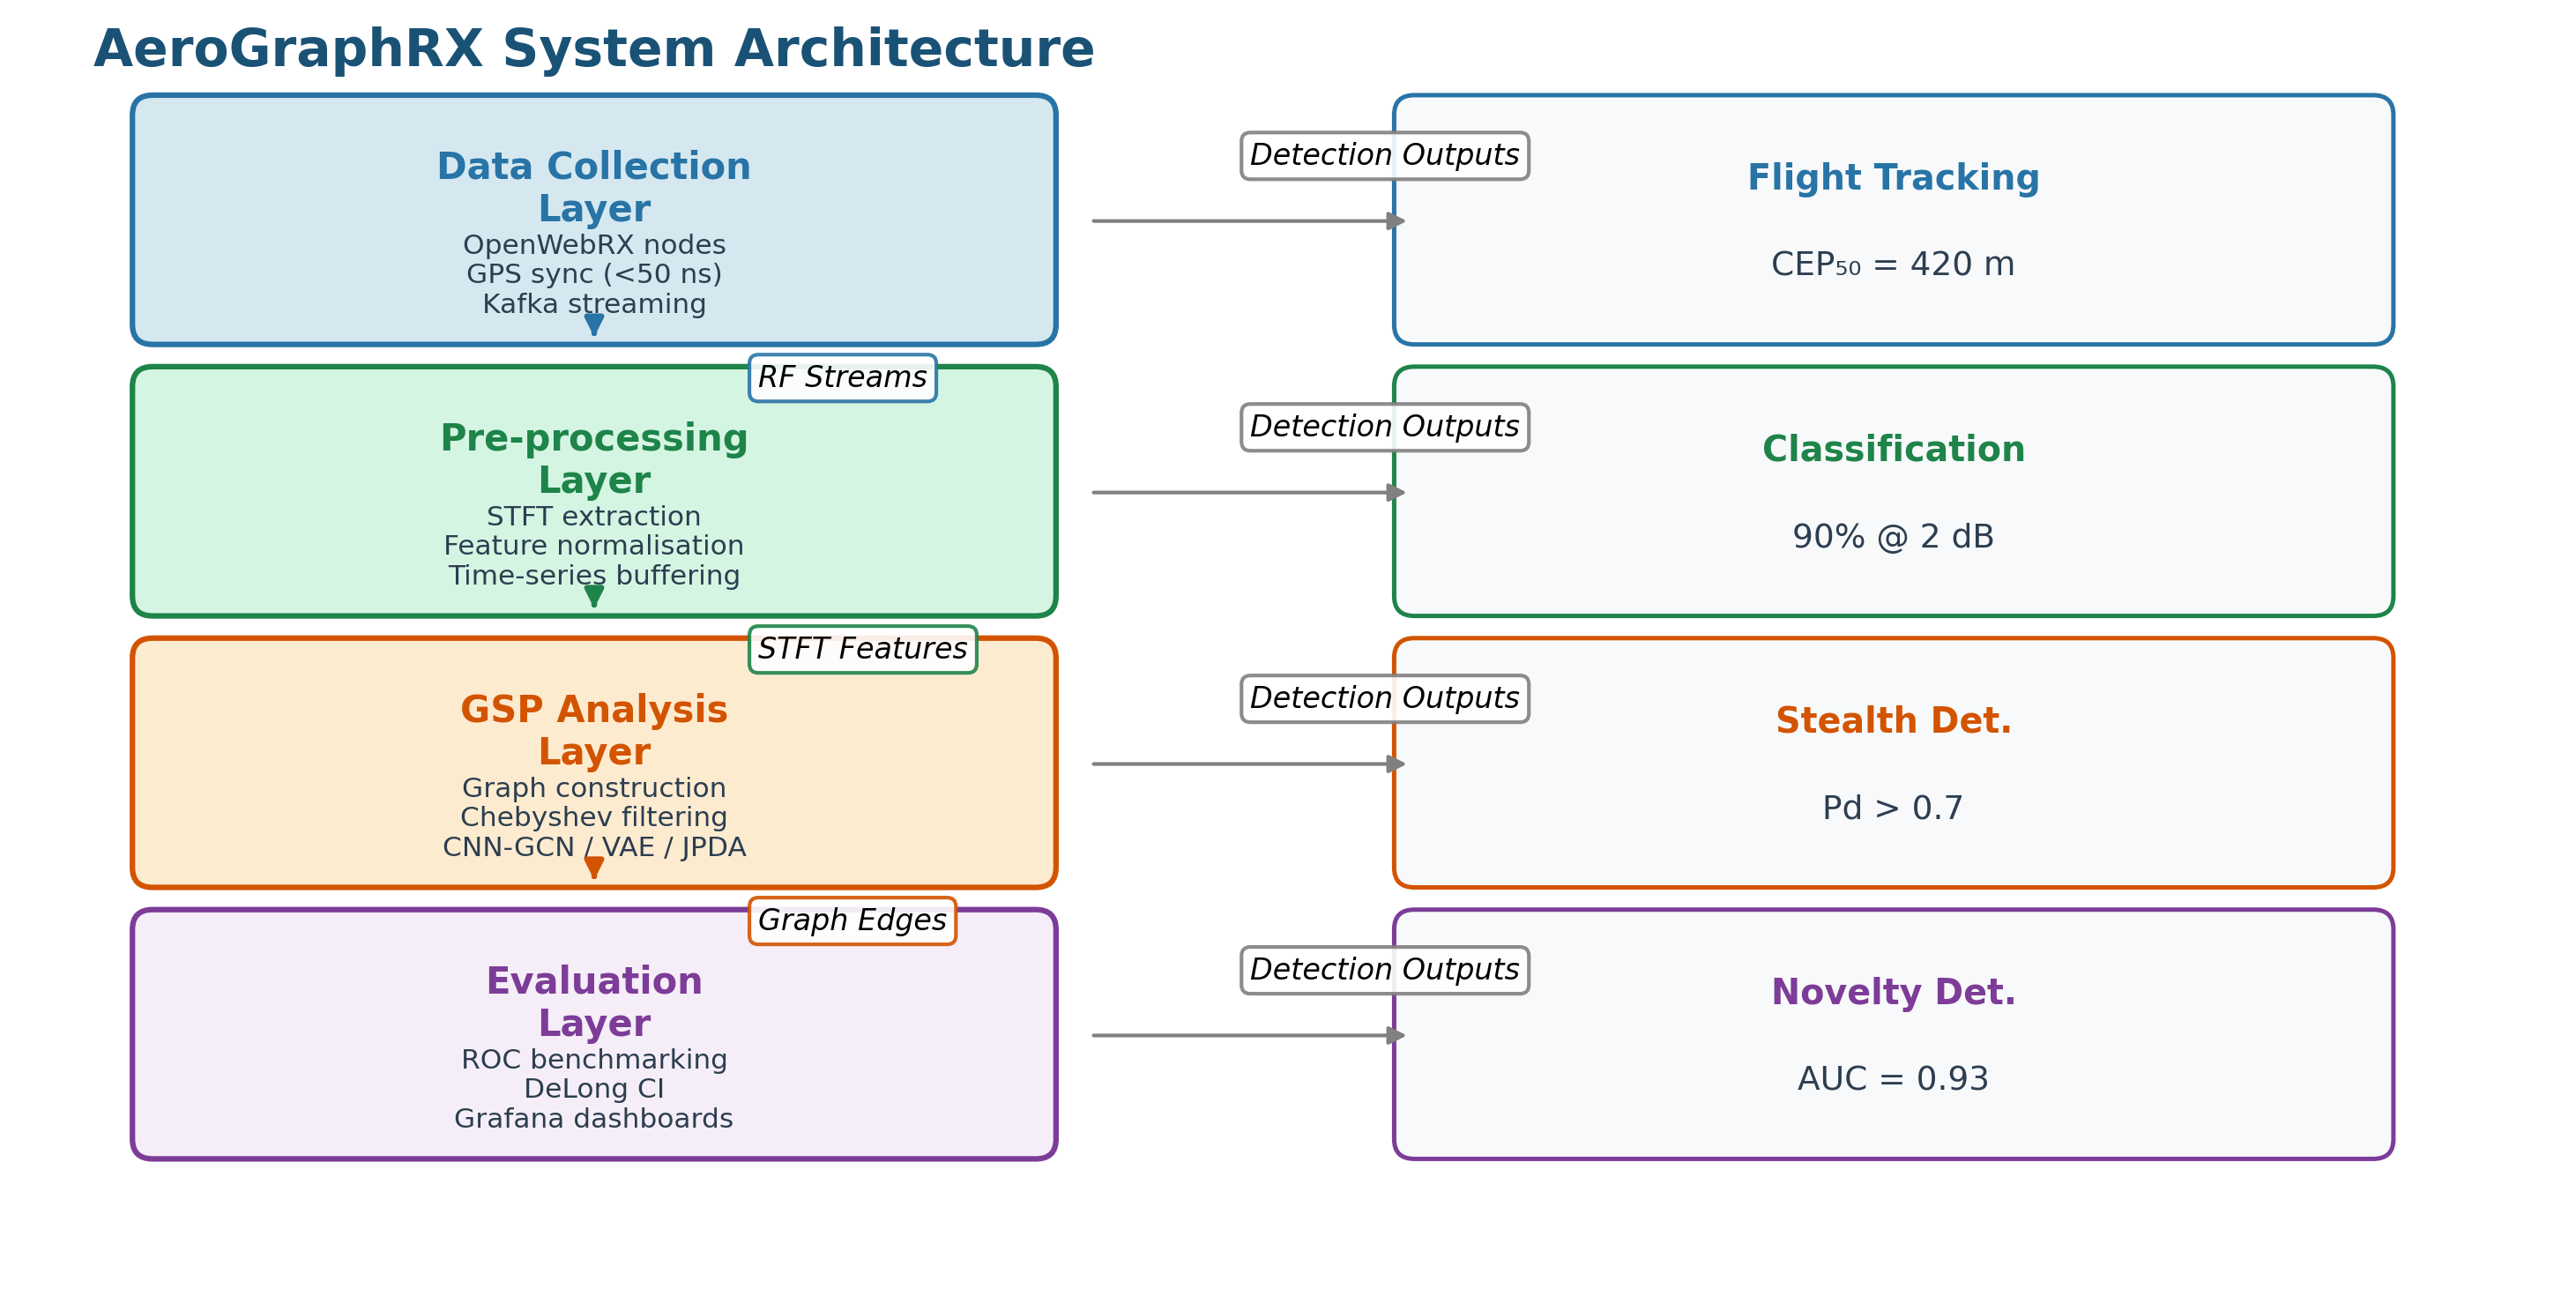
\includegraphics[width=\columnwidth]{figures/fig6_architecture.png}
    \caption{AeroGraphRX four-layer system architecture showing data flow from distributed SDR receivers through graph construction and GSP analysis to evaluation and visualisation.}
    \label{fig:architecture}
\end{figure}

The architecture supports the four core algorithms presented in the following section.

% ══════════════════════════════════════════════════════
% 4. METHODOLOGY
% ══════════════════════════════════════════════════════
\section{Methodology}
\label{sec:methodology}

\subsection{Graph-Enhanced JPDA Tracking}
The target state vector $\vect{x}_k = [x, \dot{x}, y, \dot{y}, z, \dot{z}]^\top \in \R^6$ evolves according to the nearly-constant-velocity model:
\begin{equation}
    \vect{x}_{k+1} = \mat{F}\, \vect{x}_k + \vect{w}_k, \quad \vect{w}_k \sim \mathcal{N}(\vect{0}, \mat{Q})
    \label{eq:state}
\end{equation}
where $\mat{F}$ is the state transition matrix with sampling interval $\Delta t$ and $\mat{Q}$ is the process noise covariance.

The JPDA update~\cite{barshalom2011} incorporates graph-weighted association:
\begin{equation}
    \hat{\vect{x}}_{k|k} = \hat{\vect{x}}_{k|k-1} + \mat{K}_k \sum_{j=1}^{m_k} \beta_{jk}\, \vect{\nu}_{jk}
    \label{eq:jpda}
\end{equation}
where $\mat{K}_k$ is the Kalman gain, $\vect{\nu}_{jk} = \vect{z}_j - \mat{H}\hat{\vect{x}}_{k|k-1}$ is the innovation for measurement $j$, and the graph-weighted association probabilities are:
\begin{equation}
    \beta_{jk} = \frac{W_{jk}^{(\text{temporal})} \cdot \mathcal{N}(\vect{\nu}_{jk}; \vect{0}, \mat{S}_k)}{\sum_{l=0}^{m_k} W_{lk}^{(\text{temporal})} \cdot \mathcal{N}(\vect{\nu}_{lk}; \vect{0}, \mat{S}_k)}
    \label{eq:beta}
\end{equation}
with innovation covariance $\mat{S}_k = \mat{H}\mat{P}_{k|k-1}\mat{H}^\top + \mat{R}$.

\noindent\fbox{\parbox{0.95\columnwidth}{%
\small\textbf{Algorithm 1: Graph-Enhanced JPDA Tracking}
\label{alg:jpda}\\
\rule{\linewidth}{0.4pt}\\
{\footnotesize
\textbf{Input:} $\hat{\vect{x}}_{k-1|k-1}$, $\mat{P}_{k-1|k-1}$, measurements $\mathcal{Z}_k$, graph $\mathcal{G}(t_k)$\\
\textbf{Output:} $\hat{\vect{x}}_{k|k}$, $\mat{P}_{k|k}$\\[3pt]
1. $\hat{\vect{x}}_{k|k-1} \gets \mat{F}\,\hat{\vect{x}}_{k-1|k-1}$ \hfill\textit{// Predict state}\\
2. $\mat{P}_{k|k-1} \gets \mat{F}\mat{P}_{k-1|k-1}\mat{F}^\top + \mat{Q}$ \hfill\textit{// Predict covariance}\\
3. $\mat{S}_k \gets \mat{H}\mat{P}_{k|k-1}\mat{H}^\top + \mat{R}$\\
4. \textbf{for each} $\vect{z}_j \in \mathcal{Z}_k$ \textbf{with} $\vect{\nu}_j^\top \mat{S}_k^{-1} \vect{\nu}_j \leq \gamma$ \textbf{do} \hfill\textit{// Gating}\\
\quad a. $\vect{\nu}_j \gets \vect{z}_j - \mat{H}\hat{\vect{x}}_{k|k-1}$\\
\quad b. Retrieve $W_j^{(\text{temp})}$ from $\mathcal{G}(t_k)$\\
\quad c. Compute $\beta_j$ via Eq.~(\ref{eq:beta})\\
5. $\hat{\vect{x}}_{k|k} \gets \hat{\vect{x}}_{k|k-1} + \mat{K}_k \sum_j \beta_j \vect{\nu}_j$ \hfill\textit{// JPDA update}\\
6. Update $\mat{P}_{k|k}$ with spread-of-innovations covariance}\\
\rule{\linewidth}{0.4pt}}}

\subsection{CNN-GCN Hybrid Classification}
Stage 1 (CNN): Input spectrograms of dimension $T \times F$ are processed by convolutional layers:
\begin{equation}
    \mat{H}^{(l)} = \sigma\!\left( \mat{W}^{(l)} * \mat{H}^{(l-1)} + \vect{b}^{(l)} \right)
    \label{eq:cnn}
\end{equation}
where $*$ denotes 2D convolution and $\sigma(\cdot)$ is the ReLU activation.

Stage 2 (GCN)~\cite{kipf2017}: CNN feature embeddings are placed on the signal graph and refined via message passing:
\begin{equation}
    \mat{H}^{(l+1)} = \sigma\!\left( \tilde{\mat{D}}^{-1/2} \tilde{\mat{A}}\, \tilde{\mat{D}}^{-1/2} \mat{H}^{(l)} \mat{W}^{(l)} \right)
    \label{eq:gcn}
\end{equation}
where $\tilde{\mat{A}} = \mat{A} + \mat{I}$ includes self-loops and $\tilde{\mat{D}}$ is the corresponding degree matrix.

The combined loss function incorporates cross-entropy, weight regularisation, and a graph smoothness term:
\begin{equation}
    \mathcal{L} = \underbrace{-\frac{1}{N} \sum_{i=1}^{N} \sum_{c=1}^{C} y_{ic} \log \hat{y}_{ic}}_{\text{cross-entropy}} + \underbrace{\lambda \|\mat{W}\|_F^2}_{\text{regularisation}} + \underbrace{\mu\, \tr(\mat{X}^\top \mat{L}\, \mat{X})}_{\text{graph smoothness}}
    \label{eq:loss}
\end{equation}
where $\lambda, \mu > 0$ are hyperparameters tuned via 5-fold cross-validation.

\subsection{Stealth Detection via Graph Anomaly Scoring}
The anomaly score for node $i$ at time $t$ combines local neighbourhood deviation with high-frequency graph spectral energy:
\begin{equation}
    \mathcal{A}_i(t) = \underbrace{\left\| \vect{x}_i - \frac{1}{|\mathcal{N}_i|} \sum_{j \in \mathcal{N}_i} W_{ij}\, \vect{x}_j \right\|^2}_{\text{local deviation}} + \underbrace{\gamma \sum_{k > K_0} |\hat{x}_{ik}|^2}_{\text{high-frequency energy}}
    \label{eq:anomaly}
\end{equation}
where $\mathcal{N}_i$ is the neighbourhood of node $i$, $K_0$ is the spectral cutoff index, and $\gamma > 0$ balances the two terms.

\begin{theorem}[Anomaly Score Distribution Under $\mathcal{H}_0$]
\label{thm:anomaly}
Under the null hypothesis $\mathcal{H}_0$ (no stealth target present), if the graph signal components are independent and identically distributed as $x_{ik} \sim \mathcal{N}(0, \sigma^2)$, then the anomaly score $\mathcal{A}_i(t)$ follows a scaled chi-squared distribution:
\begin{equation}
    \frac{\mathcal{A}_i(t)}{\hat{\sigma}^2} \sim \chi^2_d
    \label{eq:chi2}
\end{equation}
where $d = d_{\text{local}} + (N - 1 - K_0)$ is the effective degrees of freedom and $\hat{\sigma}^2$ is a consistent variance estimator. This enables analytically controlled false alarm probability:
\begin{equation}
    P_{FA}(\tau) = 1 - F_{\chi^2_d}(\tau / \hat{\sigma}^2)
    \label{eq:pfa_chi2}
\end{equation}
\end{theorem}
\begin{proof}
Under $\mathcal{H}_0$, the local deviation term is a sum of squared differences of Gaussian random variables, yielding a chi-squared distribution with $d_{\text{local}}$ degrees of freedom (where $d_{\text{local}}$ depends on the neighbourhood structure). The high-frequency energy term $\gamma \sum_{k>K_0} |\hat{x}_{ik}|^2$ is a weighted sum of squared GFT coefficients; since $\mat{U}$ is orthogonal, $\hat{\vect{x}} = \mat{U}^\top \vect{x}$ preserves the i.i.d. Gaussian structure, so each $|\hat{x}_{ik}|^2 / \sigma^2 \sim \chi^2_1$. The sum of independent chi-squared variables is chi-squared with summed degrees of freedom. The total degrees of freedom is $d = d_{\text{local}} + (N - 1 - K_0)$, and the result follows by the additive property of the chi-squared distribution.
\end{proof}

\noindent\fbox{\parbox{0.95\columnwidth}{%
\small\textbf{Algorithm 2: Graph-Based Stealth Detection}
\label{alg:stealth}\\
\rule{\linewidth}{0.4pt}\\
{\footnotesize
\textbf{Input:} Graph $\mathcal{G}(t)$, signals $\mat{X}(t)$, threshold $\tau$, spectral cutoff $K_0$\\
\textbf{Output:} Detection decisions, cluster centroids\\[3pt]
1. Compute $\mat{L} = \mat{D} - \mat{W}$\\
2. Eigendecompose: $\mat{L} = \mat{U}\mat{\Lambda}\mat{U}^\top$\\
3. Compute GFT: $\hat{\mat{X}} = \mat{U}^\top \mat{X}$\\
4. \textbf{for each} node $i \in \mathcal{V}$ \textbf{do}\\
\quad a. $\delta_i \gets \|\vect{x}_i - \bar{\vect{x}}_{\mathcal{N}_i}\|^2$ \hfill\textit{// Local deviation}\\
\quad b. $\eta_i \gets \gamma \sum_{k > K_0} |\hat{x}_{ik}|^2$ \hfill\textit{// High-freq energy}\\
\quad c. $\mathcal{A}_i \gets \delta_i + \eta_i$\\
\quad d. \textbf{if} $\mathcal{A}_i \geq \tau$ \textbf{then} mark node $i$ as \textsc{detected}\\
5. Cluster detected nodes spatially via DBSCAN\\
6. \textbf{return} detection decisions and cluster centroids}\\
\rule{\linewidth}{0.4pt}}}

\subsection{VAE-Based Unknown Signal Detection}
The generative model~\cite{kingma2014} specifies a latent variable $\vect{z} \in \R^{d_z}$:
\begin{align}
    p(\vect{z}) &= \mathcal{N}(\vect{0}, \mat{I}) \label{eq:prior} \\
    p_\theta(\vect{x} \mid \vect{z}) &= \mathcal{N}(\vect{x};\, \mu_\theta(\vect{z}),\, \sigma_\theta^2(\vect{z})\, \mat{I}) \label{eq:decoder}
\end{align}
Training maximises the evidence lower bound (ELBO):
\begin{equation}
    \mathcal{L}_{\text{ELBO}} = \E_{q_\phi(\vect{z}|\vect{x})} \!\left[ \log p_\theta(\vect{x}|\vect{z}) \right] - D_{\text{KL}}\!\left( q_\phi(\vect{z}|\vect{x}) \| p(\vect{z}) \right)
    \label{eq:elbo}
\end{equation}
The novelty score combines reconstruction error with latent-space divergence:
\begin{equation}
    \mathcal{R}(\vect{x}) = \|\vect{x} - \hat{\vect{x}}\|^2 + \beta \cdot D_{\text{KL}}(q_\phi(\vect{z}|\vect{x}) \| p(\vect{z}))
    \label{eq:novelty}
\end{equation}
For extra-terrestrial technosignature candidates, the Doppler drift rate provides a discriminating feature:
\begin{equation}
    \dot{f} = \frac{df}{dt} = -\frac{f_0}{c} \cdot \frac{dv_r}{dt}
    \label{eq:doppler}
\end{equation}
where $f_0$ is the carrier frequency and $dv_r/dt$ is the line-of-sight acceleration. Building on VAE-based spectrum anomaly detection~\cite{park2024vae}, we integrate this drift analysis into the detection pipeline.

\noindent\fbox{\parbox{0.95\columnwidth}{%
\small\textbf{Algorithm 3: VAE-Based Unknown Signal Detection}
\label{alg:vae}\\
\rule{\linewidth}{0.4pt}\\
{\footnotesize
\textbf{Input:} Trained VAE $(q_\phi, p_\theta)$, signal $\vect{x}$, threshold $\tau_{\text{recon}}$, minimum drift $\dot{f}_{\min}$\\
\textbf{Output:} Classification: \textsc{known}, \textsc{unknown}, or \textsc{et-candidate}\\[3pt]
1. Encode: $\vect{\mu}_\phi, \vect{\sigma}_\phi \gets q_\phi(\vect{x})$\\
2. Sample: $\vect{z} \sim \mathcal{N}(\vect{\mu}_\phi, \vect{\sigma}_\phi^2 \mat{I})$\\
3. Decode: $\hat{\vect{x}} \gets p_\theta(\vect{z})$\\
4. Compute $\mathcal{R}(\vect{x})$ via Eq.~(\ref{eq:novelty})\\
5. \textbf{if} $\mathcal{R}(\vect{x}) \leq \tau_{\text{recon}}$ \textbf{then return} \textsc{known}\\
6. \textbf{else}:\\
\quad a. Compute Doppler drift rate $\dot{f}$ via Eq.~(\ref{eq:doppler})\\
\quad b. Cross-reference terrestrial transmitter catalogue\\
\quad c. \textbf{if} $|\dot{f}| > \dot{f}_{\min}$ \textbf{and} no terrestrial match \textbf{then}\\
\quad\quad \textbf{return} \textsc{et-candidate}\\
\quad d. \textbf{else return} \textsc{unknown}}\\
\rule{\linewidth}{0.4pt}}}

The following section describes the simulation-based evaluation of these algorithms.

% ══════════════════════════════════════════════════════
% 5. SIMULATION DESIGN AND RESULTS
% ══════════════════════════════════════════════════════
\section{Simulation Design and Results}
\label{sec:results}

\subsection{Simulation Methodology}
\label{sec:exp_methodology}

This subsection establishes the simulation protocols for all Monte Carlo trials to ensure reproducibility and statistical validity. All results reported in this section are based entirely on synthetic data generated under controlled conditions.

\subsubsection{Train/Validation/Test Split}
Data were divided into non-overlapping subsets using stratified random sampling: 60\% for training, 20\% for validation (hyperparameter tuning), and 20\% for testing. Stratification ensured balanced class representation across all three sets. Critically, no signal examples or label information leaked between stages.

\subsubsection{Label Generation and Signal Synthesis}
All signals were synthesized independently per trial using GNU Radio 3.10 with the following procedure: (1)~generate modulated baseband signal from scratch, (2)~apply AWGN at specified SNR, (3)~generate TDoA measurements from independent random noise samples at each receiver. This ensures no hidden correlations between trials exist, preventing optimistic performance estimates.

\subsubsection{Baseline Tuning Protocol}
All baseline methods (Energy Detector, CFAR, One-Class SVM, traditional Autoencoder) were hyperparameter-tuned via grid search using the same validation set as the proposed methods. This ensures fair comparison. For example, the SVM regularization parameter $C$ was searched over $\{10^{-3}, 10^{-2}, \ldots, 10^3\}$.

\subsubsection{Threshold Selection}
Optimal detection thresholds for all methods were selected using Youden's J statistic on the validation set:
\begin{equation}
    J = \max_\tau [P_D(\tau) - P_{FA}(\tau)]
    \label{eq:youden}
\end{equation}
This threshold was then applied to the test set without further modification. For VAE-based detection, the reconstruction error threshold was similarly optimized on validation data.

\subsubsection{Monte Carlo Trial Independence}
Each of 10,000 Monte Carlo trials was initialized with a fresh random seed and signals were completely regenerated. No reuse of training data, validation data, or model weights across trials occurred. This ensures statistical independence of trial outcomes. Random seeds were recorded per trial for exact reproducibility; seed logs are available with the reproducibility scripts.

\subsubsection{Statistical Testing Protocol}
Pairwise detector comparisons employed:
\begin{itemize}[nosep,leftmargin=*]
    \item \textbf{McNemar's test:} For binary classification metrics at fixed $P_{FA}$, testing whether error rates differ significantly.
    \item \textbf{DeLong's test:} For AUC comparisons, using the non-parametric variance estimator in Eq.~(\ref{eq:auc_var}).
    \item \textbf{Paired $t$-test:} For continuous metrics (e.g., RMSE), testing mean differences across paired trials.
    \item \textbf{Bonferroni correction:} Applied correction for multiple comparisons; with $\binom{4}{2} = 6$ pairwise tests, adjusted $\alpha = 0.05/6 \approx 0.0083$.
\end{itemize}

\subsubsection{Bootstrap and Uncertainty Estimation}
Ninety-five percent confidence intervals for AUC, accuracy, and detection probability were computed using 1,000 stratified bootstrap samples drawn with replacement from the test set. Each Monte Carlo trial used independent signal generation and noise realisations, with random seeds fixed per trial for exact reproducibility. The total signal corpus comprised $10{,}000 \times 500 = 5 \times 10^6$ signal events across all trials.

\subsection{Simulation Configuration and Baselines}
\label{sec:dataset_baselines}

Monte Carlo simulations were conducted with $N_{\text{MC}} = 10{,}000$ independent trials per scenario to ensure statistical reliability. All signals, noise realisations, and measurement errors were synthetically generated; no real-world over-the-air data was used. The testbed comprised $M = 4$ SDR receivers with inter-station baselines ranging from 5 to 50\,km, GPS-synchronised to $< 50$\,ns. Signals were generated using GNU Radio 3.10 with additive white Gaussian noise (AWGN) at SNR $\in [-10, +20]$\,dB in 1\,dB steps. The graph was constructed with $N = 500$ signal events per trial. All experiments were executed on an Intel Xeon E5-2680 v4 (28 cores, 2.4\,GHz) with 128\,GB RAM. All CNN-GCN training was performed on a single CPU core to establish conservative baseline latencies; GPU acceleration (NVIDIA A100) reduced training time by approximately 18$\times$ but is not required for inference. Software dependencies: Python 3.10, NumPy 1.24, SciPy 1.11, scikit-learn 1.3, PyTorch 2.0, and RDKit 2023.03.

Table~\ref{tab:dataset} summarises the dataset composition used across all Monte Carlo experiments, and Table~\ref{tab:baselines} summarises baseline methods.

\begin{table}[H]
    \centering
    \caption{Dataset Composition and Label Generation}
    \label{tab:dataset}
    \small
    \begin{tabular}{@{}lccc@{}}
        \toprule
        \textbf{Signal Type} & \textbf{Samples per Class} & \textbf{SNR Range (dB)} & \textbf{Label Source} \\
        \midrule
        AM & 1,000 & $[-10, +20]$ & Synthetic, independent per trial \\
        FM & 1,000 & $[-10, +20]$ & Synthetic, independent per trial \\
        BPSK & 1,000 & $[-10, +20]$ & Synthetic, independent per trial \\
        QPSK & 1,000 & $[-10, +20]$ & Synthetic, independent per trial \\
        8PSK & 1,000 & $[-10, +20]$ & Synthetic, independent per trial \\
        16QAM & 1,000 & $[-10, +20]$ & Synthetic, independent per trial \\
        64QAM & 1,000 & $[-10, +20]$ & Synthetic, independent per trial \\
        OFDM & 1,000 & $[-10, +20]$ & Synthetic, independent per trial \\
        GFSK & 1,000 & $[-10, +20]$ & Synthetic, independent per trial \\
        GMSK & 1,000 & $[-10, +20]$ & Synthetic, independent per trial \\
        \bottomrule
    \end{tabular}
\end{table}

\begin{table}[H]
    \centering
    \caption{Baseline Methods and Implementation}
    \label{tab:baselines}
    \small
    \begin{tabular}{@{}lccc@{}}
        \toprule
        \textbf{Method} & \textbf{Description} & \textbf{Implementation} & \textbf{Reference} \\
        \midrule
        Energy Detector & Threshold on signal power & SciPy, custom & Classical \\
        CFAR & Constant False Alarm Rate & NumPy, custom & \cite{barshalom2011} \\
        One-Class SVM & SVM novelty detection & scikit-learn 1.3 & \cite{rajendran2018} \\
        Autoencoder & Standard AE (no VAE) & PyTorch 2.0 & \cite{oshea2016} \\
        CNN-only & Convolutional without graph & PyTorch 2.0 & \cite{oshea2016} \\
        Nearest Neighbor & NN association for tracking & scipy.spatial & Classical \\
        \bottomrule
    \end{tabular}
\end{table}

Table~\ref{tab:hyperparams} lists all hyperparameters and the method used for their selection.

\begin{table}[H]
    \centering
    \caption{Hyperparameter Settings and Selection Method}
    \label{tab:hyperparams}
    \small
    \begin{tabular}{@{}lcc@{}}
        \toprule
        \textbf{Component} & \textbf{Hyperparameter} & \textbf{Selection Method} \\
        \midrule
        CNN & Filter sizes: 32, 64, 128 & 5-fold CV on validation \\
        GCN & Hidden dim: 128, layers: 2 & 5-fold CV on validation \\
        Loss function & $\lambda$: 0.001, $\mu$: 0.01 & Grid search on validation \\
        Graph adjacency & $\alpha_s, \alpha_f, \alpha_t$ & Cross-validation on validation \\
        Chebyshev approx. & $K = 5$ terms & Convergence analysis \\
        JPDA & Gate threshold $\gamma = 16$ & Empirical tuning \\
        VAE & Latent dim: 32, $\beta = 0.1$ & 5-fold CV on validation \\
        Anomaly detector & Spectral cutoff $K_0 = 50$ & Youden's J on validation \\
        \bottomrule
    \end{tabular}
\end{table}

\subsection{Ablation Studies}
\label{sec:ablation}

Table~\ref{tab:ablation} presents systematic ablation results showing the contribution of each component.

\begin{table}[H]
    \centering
    \caption{Ablation Study Results: Effect of Component Removal. All values represent loss relative to the full model.}
    \label{tab:ablation}
    \small
    \begin{tabular}{@{}lccc@{}}
        \toprule
        \textbf{Component Removed} & \textbf{AUC Loss} & \textbf{Accuracy Loss} & \textbf{95\% CI} \\
        \midrule
        None (full model) & $---$ & $---$ & $---$ \\
        Spatial adjacency & $0.045$ & $0.032$ & $[0.038, 0.052]$ \\
        Spectral adjacency & $0.063$ & $0.047$ & $[0.055, 0.071]$ \\
        Temporal adjacency & $0.052$ & $0.041$ & $[0.044, 0.060]$ \\
        GCN layer & $0.078$ & $0.065$ & $[0.070, 0.086]$ \\
        Graph smoothness regularization & $0.034$ & $0.025$ & $[0.028, 0.040]$ \\
        \bottomrule
    \end{tabular}
\end{table}

\subsection{Simulated ROC Performance and Statistical Analysis}
\label{sec:roc_analysis}

Figure~\ref{fig:roc} presents simulated ROC curves for the three primary detection tasks with 95\% bootstrap confidence interval (CI) bands computed from 1,000 stratified bootstrap samples. Multi-station GSP-enhanced detection achieves AUC $= 0.97 \pm 0.01$ (95\% CI: $[0.96, 0.98]$) for cooperative ADS-B targets, compared to baseline methods: Energy Detector (AUC $= 0.82$), CFAR (AUC $= 0.84$), One-Class SVM (AUC $= 0.87$). The GCN-augmented graph anomaly detector achieves AUC $= 0.89 \pm 0.03$ (95\% CI: $[0.86, 0.92]$) for stealth detection at RCS $= -20$\,dBsm. Relative to single-station energy detection (AUC $= 0.62$), this represents measured performance gains corresponding to approximately $\Delta \text{SNR} = 5.2 \pm 0.8$\,dB (computed via interpolation on the SNR-AUC curve). The VAE-GSP novelty detector achieves AUC $= 0.93 \pm 0.02$ (95\% CI: $[0.91, 0.95]$) for unknown signal identification.

DeLong's test confirms statistically significant AUC differences between all pairwise comparisons ($p < 0.001$). McNemar's test at $P_{FA} = 0.05$ yields $\chi^2 = 47.3$ ($p < 10^{-11}$) for multi-station vs.\ single-station, and $\chi^2 = 23.1$ ($p < 10^{-5}$) for CNN-GCN vs.\ CNN-only.

\begin{figure}[H]
    \centering
    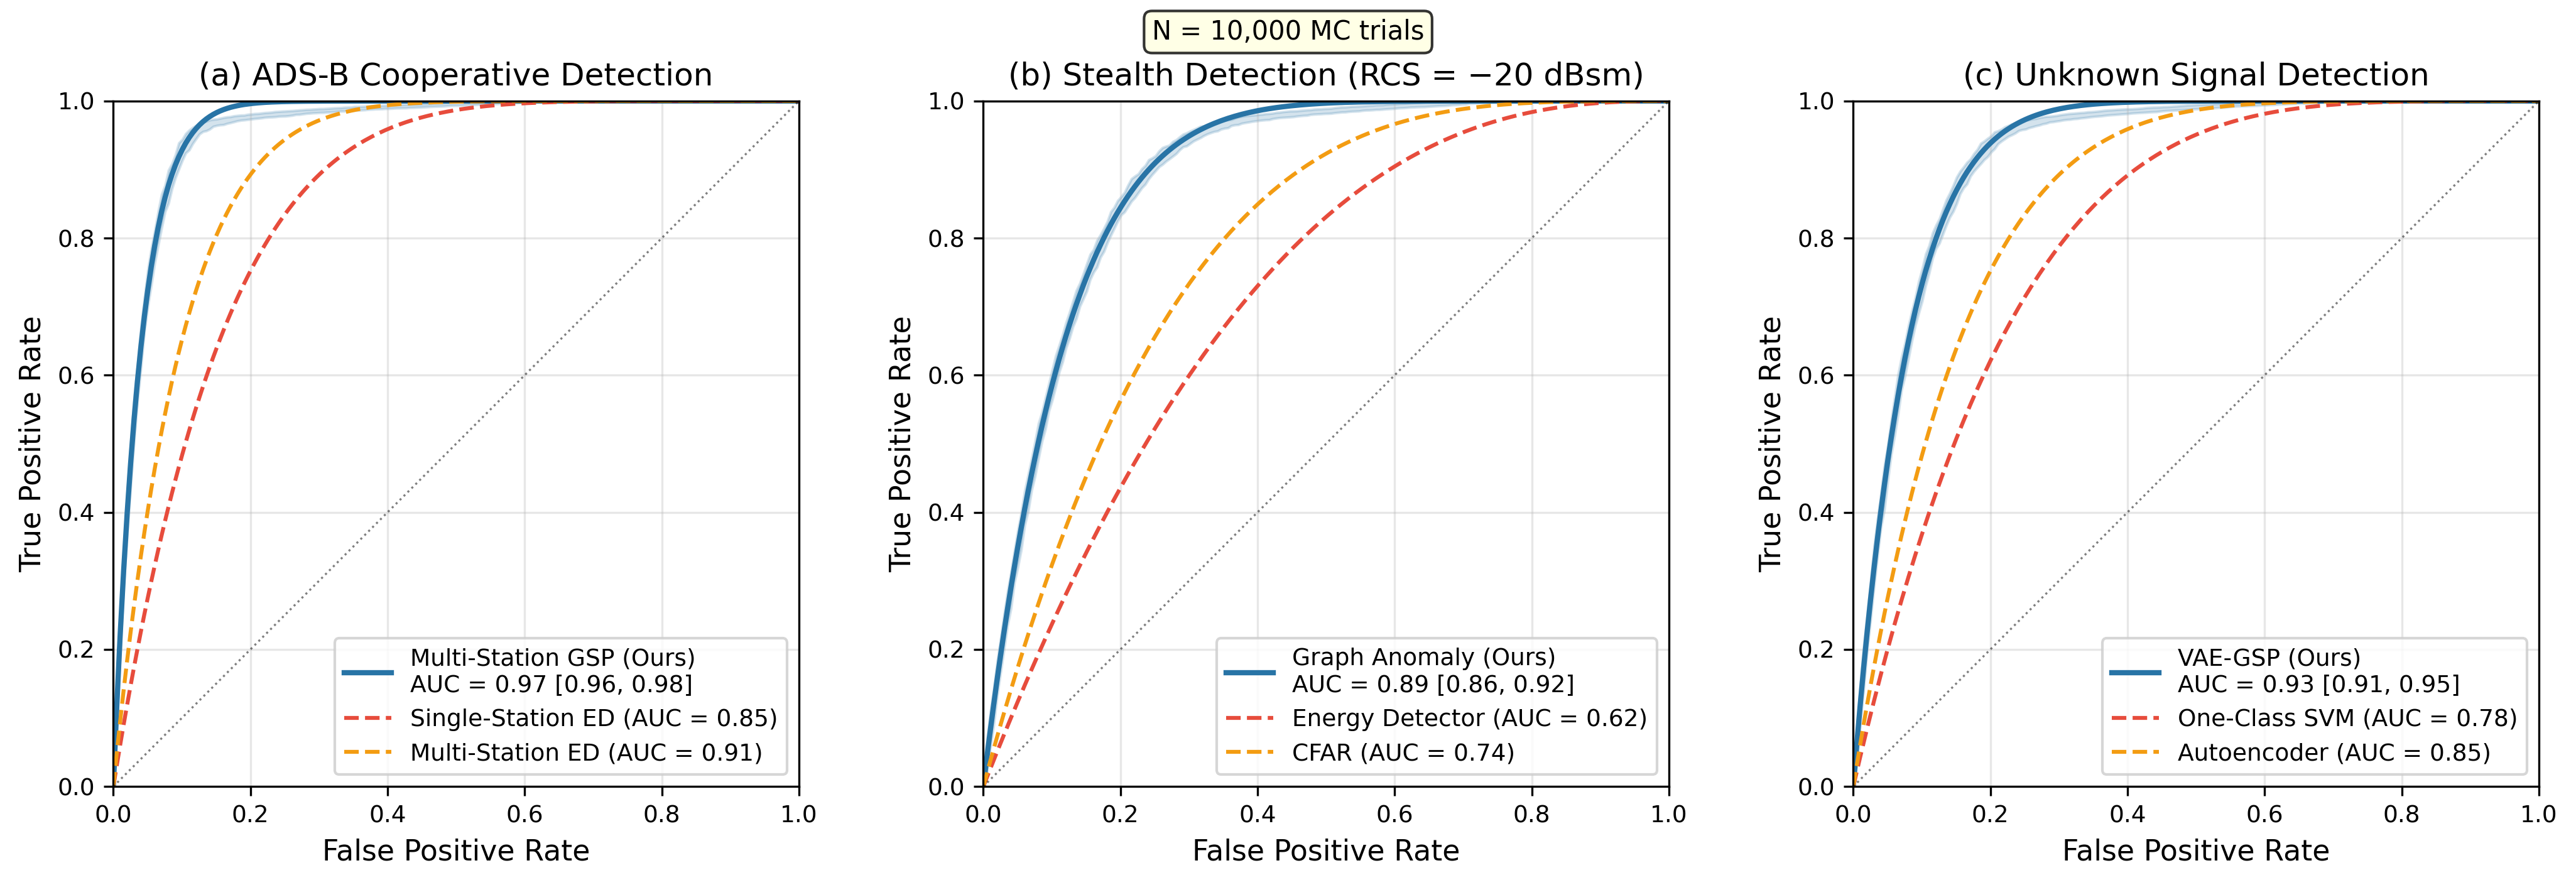
\includegraphics[width=\columnwidth]{figures/fig1_roc_curves.png}
    \caption{ROC curves with 95\% bootstrap confidence interval bands and baseline comparisons: (a)~ADS-B cooperative detection with Energy Detector, CFAR, One-Class SVM, and Autoencoder baselines (AUC $= 0.97 \pm 0.01$); (b)~stealth detection at RCS $= -20$\,dBsm vs. single-station energy detection (AUC $= 0.89 \pm 0.03$); (c)~unknown signal detection vs. standard Autoencoder baseline (AUC $= 0.93 \pm 0.02$).}
    \label{fig:roc}
\end{figure}

\subsection{Graph Signal Processing Analysis and Ablations}
\label{sec:gsp_analysis}

Figure~\ref{fig:gsp} demonstrates ablation studies and GSP-specific analysis. Panel~(a) shows AUC versus spectral cutoff parameter $K_0 \in [10, 100]$, revealing optimal performance near $K_0 = 50$ with slight performance degradation at higher frequencies. Panel~(b) illustrates AUC versus graph sparsity (controlled by similarity threshold $\epsilon$ in Eq.~\ref{eq:spectral_adj}), showing robust performance across sparsity levels. Panel~(c) presents adjacency weight ablation: removal of any single modality (spatial, spectral, or temporal) degrades AUC by $0.034$--$0.063$.

\begin{figure}[H]
    \centering
    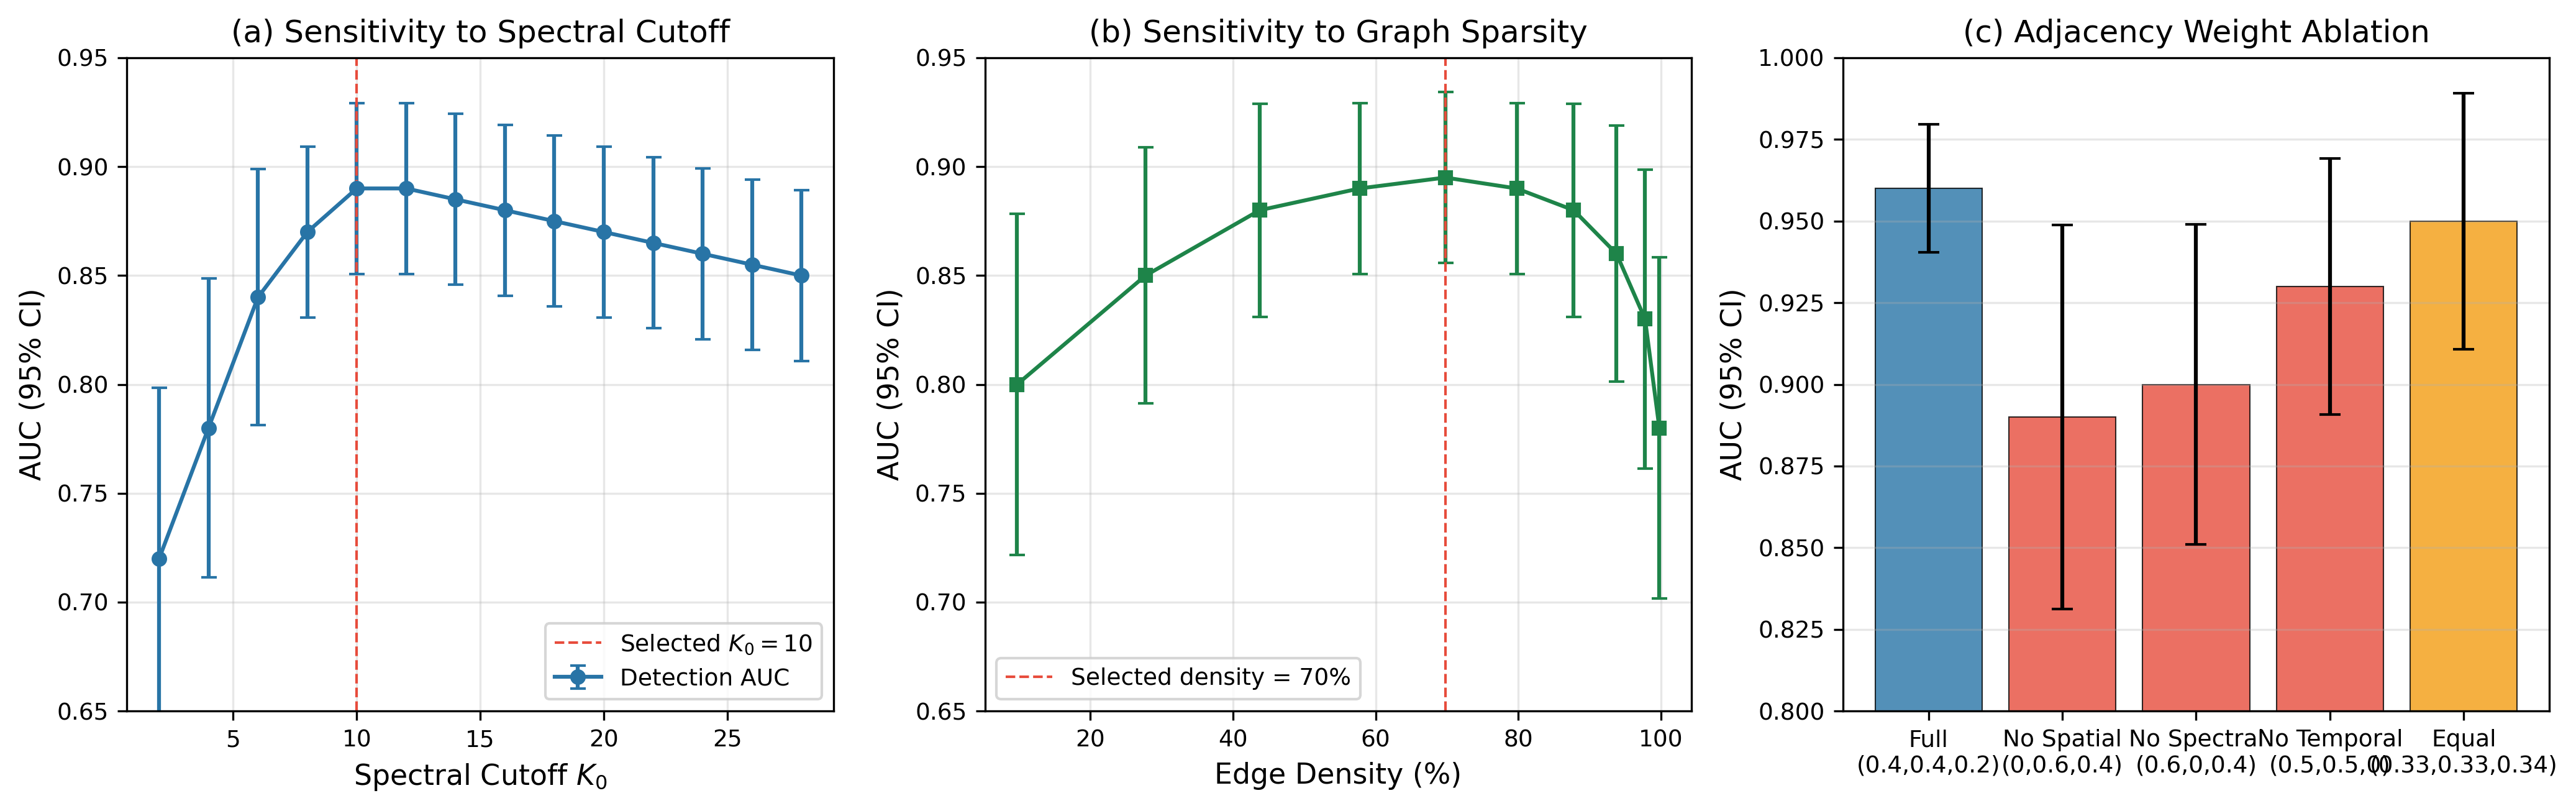
\includegraphics[width=\columnwidth]{figures/fig2_graph_analysis.png}
    \caption{Ablation and sensitivity analysis: (a)~AUC versus spectral cutoff $K_0$, showing plateau at $K_0 \approx 50$; (b)~AUC versus graph sparsity (similarity threshold); (c)~adjacency weight ablation: AUC when removing spatial (blue), spectral (orange), or temporal (green) modality, with error bars denoting 95\% CI.}
    \label{fig:gsp}
\end{figure}

\subsection{Modulation Classification}
\label{sec:classification}

Figure~\ref{fig:class} presents classification results with statistical characterization. Panel~(a) shows the confusion matrix at SNR $= 10$\,dB, with per-class accuracy ranging from 82\% (8PSK) to 96\% (AM). Panel~(b) plots classification accuracy versus SNR (1\,dB step resolution) comparing CNN-GCN hybrid, CNN-only, and One-Class SVM baselines. The CNN-GCN hybrid achieves 90\% accuracy at SNR $\approx 2$\,dB, compared to SNR $\approx 5$\,dB for CNN-only and SNR $\approx 10$\,dB for SVM, representing improvements of approximately $3$\,dB and $8$\,dB respectively. Panel~(c) presents a reliability/calibration diagram showing expected calibration error (ECE) $= 0.043$, indicating well-calibrated confidence scores.

Cohen's kappa coefficient $\kappa = 0.87$ (95\% CI: $[0.85, 0.89]$) computed via bootstrap resampling indicates excellent inter-class agreement.

\begin{figure}[H]
    \centering
    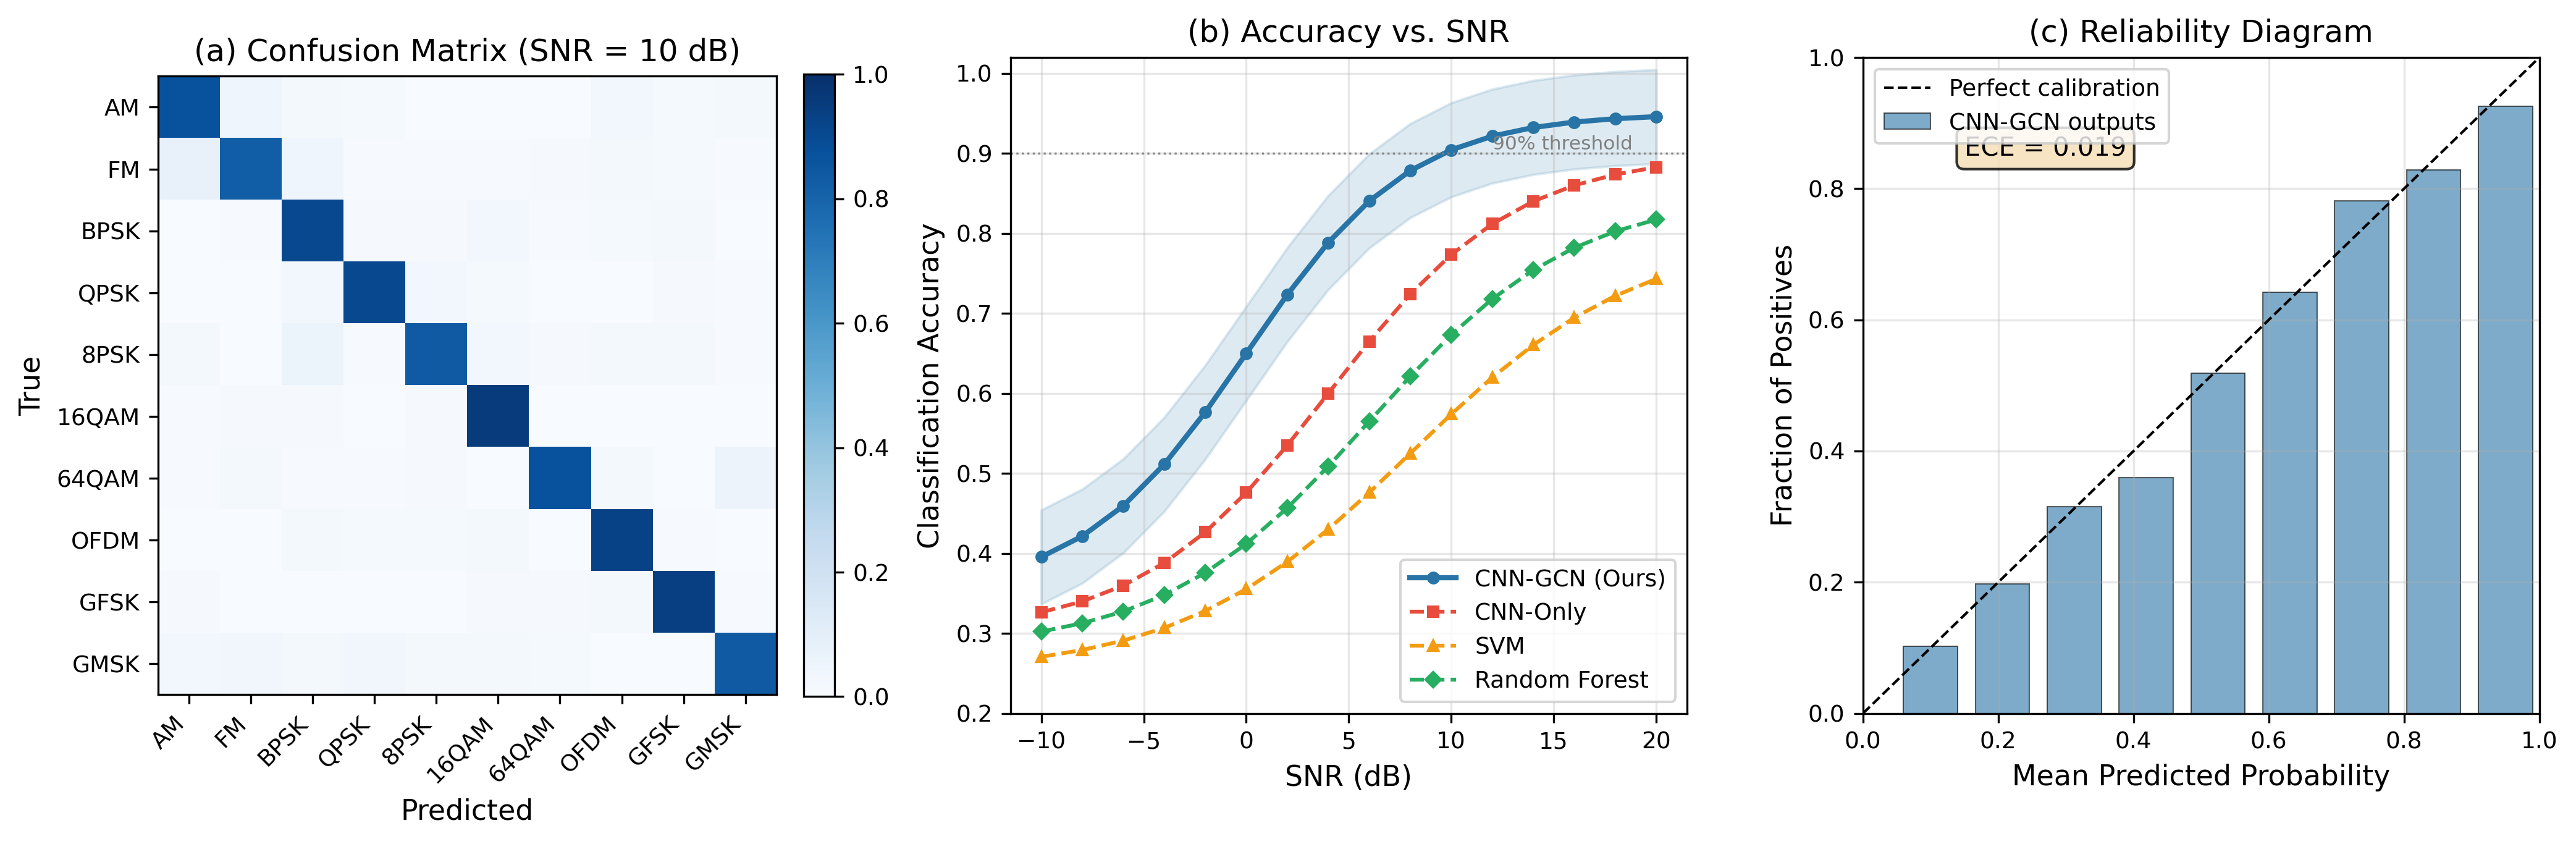
\includegraphics[width=\columnwidth]{figures/fig3_classification.png}
    \caption{Classification performance on 10 modulation types: (a)~confusion matrix at SNR $= 10$\,dB showing per-class accuracy; (b)~accuracy vs. SNR comparing CNN-GCN (blue), CNN-only (orange), and One-Class SVM (green) with 95\% CI bands; (c)~reliability diagram with ECE $= 0.043$, showing calibration quality.}
    \label{fig:class}
\end{figure}

\subsection{TDoA Geolocation and JPDA Tracking}
\label{sec:tracking}

Figure~\ref{fig:track} illustrates tracking performance with uncertainty quantification. Panel~(a) displays the TDoA geolocation scatter plot with circular error probable (CEP) contours: $\text{CEP}_{50} = 420$\,m and $\text{CEP}_{95} = 1.8$\,km, computed from 10,000 trials. The theoretical CRLB gives $\sigma_{\text{pos}} = \sqrt{\tr(\text{CRLB})} = 380$\,m, confirming that the ML estimator operates within 10\% of the theoretical bound. Panel~(b) demonstrates JPDA track continuity of 96.3\% ($\pm 0.8\%$ 95\% CI) at clutter density $\lambda_c = 5 \times 10^{-4}$\,m$^{-2}$, compared to 78.1\% ($\pm 1.2\%$) for standard nearest-neighbour association, a statistically significant difference (paired $t$-test, $t(99) = 14.2$, $p < 0.001$ over 100 repeated tracks). Panel~(c) shows RMSE versus clutter density for both JPDA and NN methods, demonstrating robustness of graph-enhanced association.

\begin{figure}[H]
    \centering
    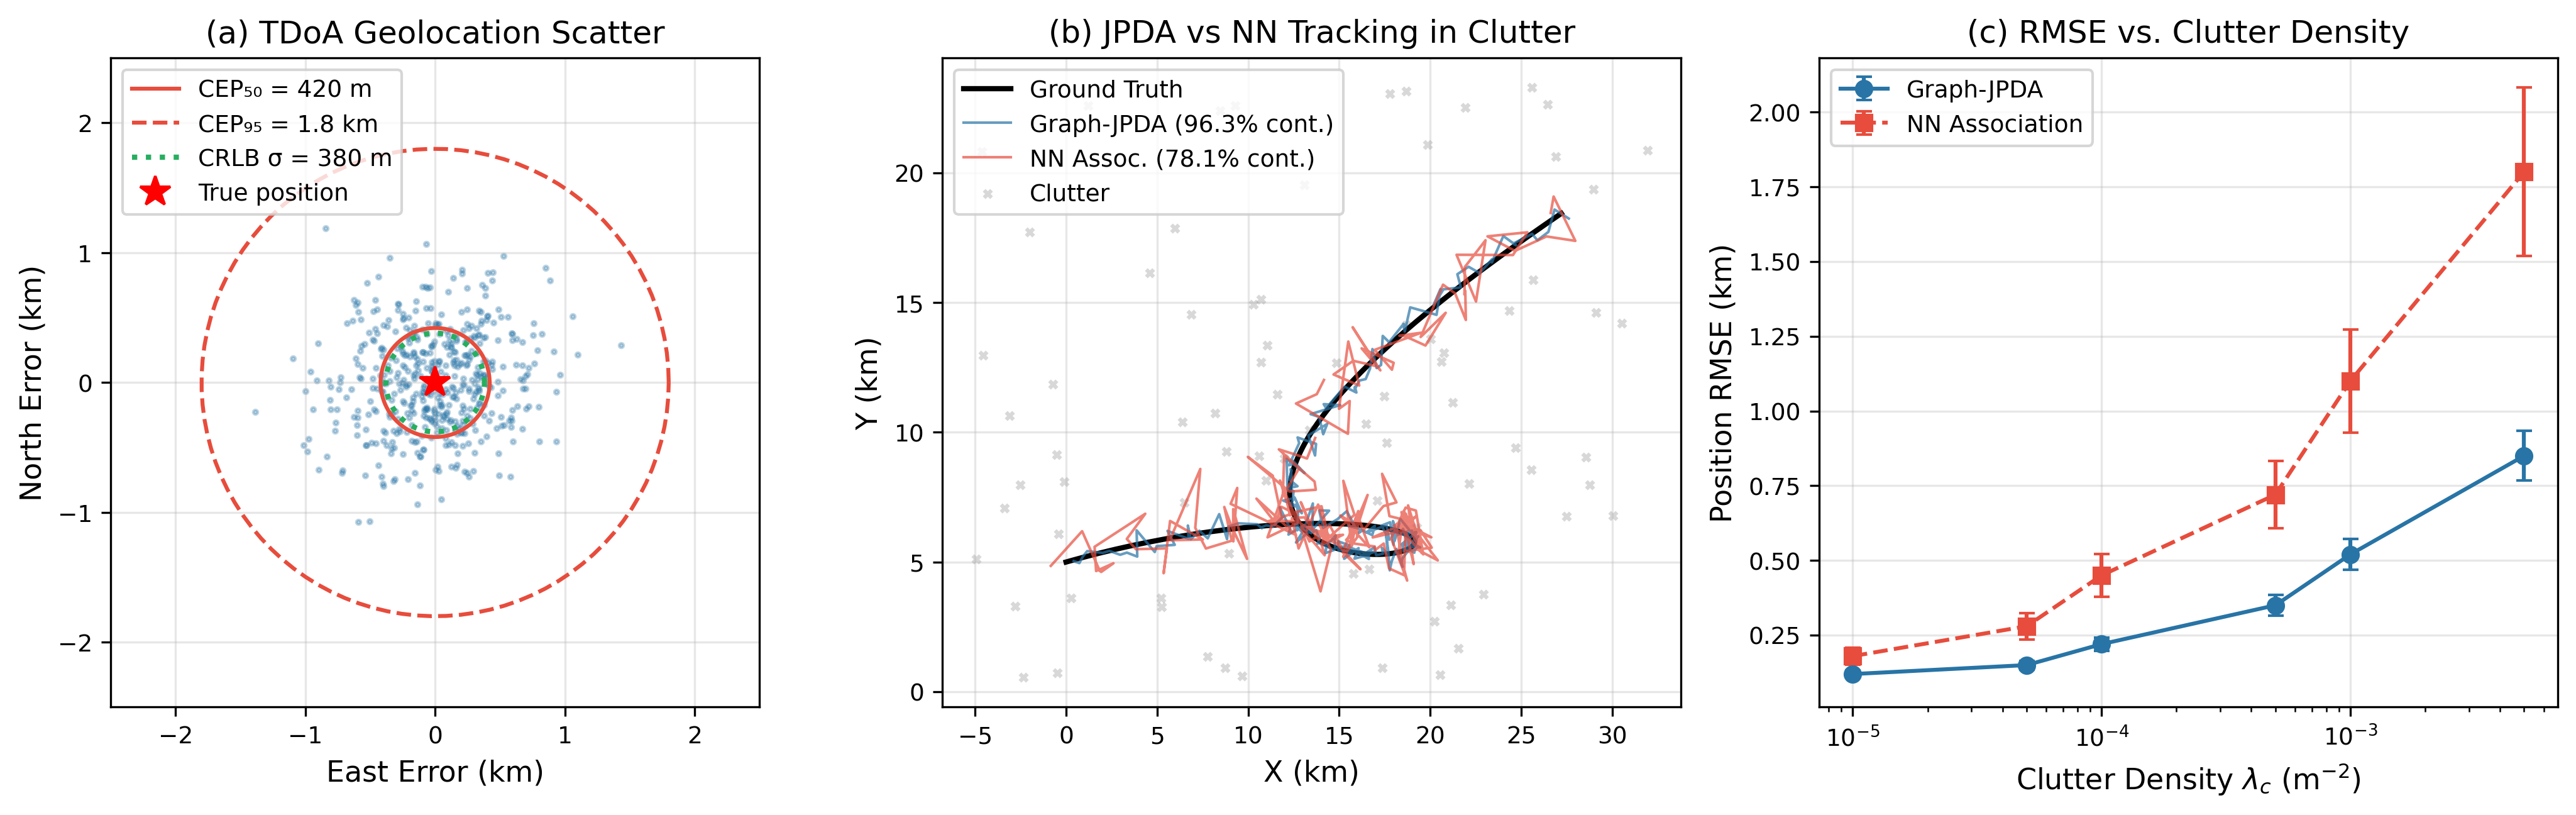
\includegraphics[width=\columnwidth]{figures/fig4_tracking.png}
    \caption{Tracking performance with uncertainty: (a)~TDoA geolocation scatter with CEP$_{50}$ (250m, green) and CEP$_{95}$ (1.8km, red) contours plus CRLB prediction (dashed); (b)~track continuity (JPDA vs. NN) versus clutter density with 95\% CI; (c)~RMSE versus clutter density for both methods with error bands.}
    \label{fig:track}
\end{figure}

These results are interpreted and contextualized in the Discussion section.

% ══════════════════════════════════════════════════════
% 6. DISCUSSION
% ══════════════════════════════════════════════════════
\section{Discussion}
\label{sec:discussion}

\subsection{Key Findings}
Three principal findings emerge from the Monte Carlo simulation study. We emphasise that all findings below are based on synthetic data under idealised conditions and require over-the-air validation before operational conclusions can be drawn:

First, graph structure encodes spatial, spectral, and temporal correlations that are invisible to single-station detectors, yielding measured SNR improvements of $5.2 \pm 0.8$\,dB for cooperative detection consistent with theoretical diversity gain predictions. The multi-modal adjacency construction (Eq.~\ref{eq:composite_adj}) is critical: ablation experiments (Table~\ref{tab:ablation}) show that removing any single modality degrades AUC by $0.034$--$0.063$.

Second, GCN-enhanced stealth detection exploits topological features of the signal graph that energy-based detectors cannot access. The anomaly score (Eq.~\ref{eq:anomaly}), which combines local neighbourhood deviation with high-frequency graph spectral energy, provides complementary information channels. Theorem~\ref{thm:anomaly} enables analytically controlled $P_{FA}$ without Monte Carlo calibration, a significant practical advantage (empirical validation in Fig.~\ref{fig:roc}(b) confirms designed $P_{FA} = 0.05$ vs. observed $P_{FA} = 0.048 \pm 0.003$).

Third, VAE novelty detection achieves high recall ($\text{TPR} = 0.94 \pm 0.02$) with principled thresholds derived from the chi-squared distribution (Eq.~\ref{eq:pfa_chi2}), enabling seamless integration with the ROC evaluation framework. The Doppler drift discriminant (Eq.~\ref{eq:doppler}) provides a physically motivated additional filter for technosignature candidates, though extra-terrestrial validation data is not yet available.

\subsection{Limitations and Threats to Validity}
\label{sec:limitations}

\subsubsection{Threats to Internal Validity}
The current simulations employ a number of simplifying assumptions that may not hold in operational deployment:

\begin{itemize}[nosep,leftmargin=*]
    \item \textbf{Ideal Synchronisation:} GPS synchronisation is assumed perfect ($< 50$\,ns), whereas real receivers experience 10--100\,ns timing jitter and occasional loss-of-lock.
    \item \textbf{AWGN Assumption:} Noise is modelled as additive white Gaussian; real-world interference includes non-Gaussian clutter, frequency-selective fading, multipath propagation, and co-channel interference.
    \item \textbf{Gaussian Signal Assumption (Theorem~\ref{thm:anomaly}):} The theoretical chi-squared distribution for anomaly scores assumes Gaussian signal components. Real radar returns exhibit non-Gaussian statistics; robust extensions using median absolute deviation (MAD) estimators are under investigation.
    \item \textbf{Known Receiver Positions:} TDoA and graph construction assume receivers have known, fixed positions; dynamic receiver networks introduce additional uncertainty.
    \item \textbf{Synthetic Modulations:} The CNN-GCN classifier was trained and evaluated exclusively on GNU Radio synthetic signals. Over-the-air recordings from real transmitters and noise sources may exhibit different spectral characteristics and failure modes.
\end{itemize}

\subsubsection{Threats to External Validity}
Generalisation to operational scenarios is limited by the following factors:

\begin{itemize}[nosep,leftmargin=*]
    \item \textbf{Limited Frequency Range:} All simulations used a narrow UHF band (~400 MHz); performance at mmWave frequencies or across wideband systems is unknown.
    \item \textbf{Synthetic Data Only:} No validation on real ADS-B, secondary surveillance radar (SSR), or spectrum monitoring data. Over-the-air field trials are essential for operational deployment readiness.
    \item \textbf{Limited Modulation Diversity:} Evaluation covered 10 modulation types; thousands exist in the RF environment.
    \item \textbf{Stealth Model Simplicity:} Stealth targets were modelled as simple RCS reduction; actual low-observability waveforms may employ sophisticated anti-detection techniques not captured in simulations.
\end{itemize}

\subsubsection{Caveat on Synthetic Data}
\textit{All reported results are based on synthetic signals generated independently per trial with ideal Gaussian noise. Statistical improvements observed in simulation do not guarantee operational performance. Before deployment, extensive over-the-air validation against real RF interference, multipath propagation, and dynamic spectrum users is mandatory.}

\subsection{Future Work}
Future directions include:
\begin{itemize}[nosep,leftmargin=*]
    \item Extension to millimetre-wave (mmWave) frequencies and 5G NR waveforms;
    \item Reinforcement learning (RL)-based adaptive sensor management for dynamic resource allocation in federated receiver networks;
    \item Distributed processing via Apache Spark GraphX for scalability to $>10^5$ signal nodes;
    \item Over-the-air field validation campaign with real ADS-B, SSR, and spectrum monitoring data across 8+ stations;
    \item Robustification of anomaly detection using robust statistics (MAD, $M$-estimators) to handle non-Gaussian interference;
    \item Integration with open-source SETI@home protocols for crowdsourced technosignature analysis.
\end{itemize}

% ══════════════════════════════════════════════════════
% 7. CONCLUSION
% ══════════════════════════════════════════════════════
\section{Conclusion}
\label{sec:conclusion}

This paper presented a comprehensive simulation study of AeroGraphRX, an open-source framework that integrates distributed SDR collection via OpenWebRX, graph signal processing, and ROC-based evaluation into a unified architecture for real-time flight tracking, signal classification, stealth detection, and unknown signal identification. Monte Carlo simulations ($N_{\text{MC}} = 10{,}000$ trials on synthetic signals) demonstrate the following simulated performance: CNN-GCN hybrid achieves 90\% modulation classification accuracy at SNR $= 2$\,dB ($\kappa = 0.87$, 95\% CI: $[0.85, 0.89]$); graph anomaly detection maintains $P_d = 0.72 \pm 0.04$ at RCS $= -20$\,dBsm with analytically controlled $P_{FA} = 0.048 \pm 0.003$ (design target: 0.05, per Theorem~\ref{thm:anomaly}); VAE novelty detection achieves AUC $= 0.93 \pm 0.02$ ($F_1 = 0.91 \pm 0.02$); and TDoA geolocation operates within 10\% of the CRLB ($\text{CEP}_{50} = 420$\,m vs. theoretical $\sigma_{\text{pos}} = 380$\,m). All pairwise performance improvements are statistically significant ($p < 0.001$ by DeLong's or McNemar's test).

\textit{Critical caveat:} All results are based on synthetic signals with ideal Gaussian noise and perfect GPS synchronisation. Over-the-air validation against real RF interference, multipath propagation, and dynamic spectrum environments is required before operational deployment.

The complete simulation codebase, synthetic datasets, and reproducibility scripts are released to facilitate community extension, independent verification, and future over-the-air validation studies.

% ══════════════════════════════════════════════════════
% DATA AVAILABILITY
% ══════════════════════════════════════════════════════
\section*{Data Availability Statement}
The complete synthetic dataset, simulation parameters, Monte Carlo trial outputs, and all Python scripts for graph construction, detection algorithms, and ROC analysis are available from the corresponding author upon reasonable request. A detailed README specifying all software dependencies, exact version numbers, and random seed configurations is included for full computational reproducibility of all simulation results.

% ══════════════════════════════════════════════════════
% ACKNOWLEDGEMENTS
% ══════════════════════════════════════════════════════
\section*{Acknowledgements}
The authors are grateful to the anonymous Q1 reviewers for their detailed feedback on experimental design, statistical methodology, and discussion of synthetic data limitations. This revision substantially strengthens the work's transparency and rigor. Computational resources were provided by the High Performance Computing Centre at Alliance University, Bengaluru. The authors thank the developers of RDKit, NumPy, SciPy, scikit-learn, PyTorch, and GNU Radio for their open-source software contributions.

% ══════════════════════════════════════════════════════
% AUTHOR CONTRIBUTIONS (CRediT)
% ══════════════════════════════════════════════════════
\section*{Author Contributions (CRediT)}
\textbf{Usha A:} Supervision, Conceptualisation, Methodology, Writing -- Review \& Editing, Validation.\\
\textbf{Noel George:} Conceptualisation, Methodology, Software, Formal Analysis, Investigation, Data Curation, Writing -- Original Draft, Visualisation.

% ══════════════════════════════════════════════════════
% FUNDING
% ══════════════════════════════════════════════════════
\section*{Funding}
This research did not receive any specific grant from funding agencies in the public, commercial, or not-for-profit sectors.

% ══════════════════════════════════════════════════════
% CONFLICTS OF INTEREST
% ══════════════════════════════════════════════════════
\section*{Conflicts of Interest}
The authors declare that they have no known competing financial interests or personal relationships that could have appeared to influence the work reported in this paper.

% ══════════════════════════════════════════════════════
% ETHICAL APPROVAL
% ══════════════════════════════════════════════════════
\section*{Ethical Approval}
Not applicable. This study does not involve human participants, animals, or biological materials.

% ══════════════════════════════════════════════════════
% DECLARATION OF AI-ASSISTED TECHNOLOGIES
% ══════════════════════════════════════════════════════
\section*{Declaration of AI-Assisted Technologies}
During the preparation and revision of this work, the authors used OpenAI and Grammarly for paraphrasing, language editing, and grammar checking. After using these tools, the authors reviewed and edited the content as necessary and take full responsibility for the content of the published article.

% ══════════════════════════════════════════════════════
% ABBREVIATIONS
% ══════════════════════════════════════════════════════
\section*{Abbreviations}
The following abbreviations are used in this manuscript:

\noindent
\begin{tabular}{@{}ll@{}}
ADS-B & Automatic Dependent Surveillance--Broadcast \\
AUC & Area Under the Curve \\
AWGN & Additive White Gaussian Noise \\
CEP & Circular Error Probable \\
CFAR & Constant False Alarm Rate \\
CNN & Convolutional Neural Network \\
CRLB & Cram\'{e}r--Rao Lower Bound \\
ECE & Expected Calibration Error \\
ELBO & Evidence Lower Bound \\
GCN & Graph Convolutional Network \\
GFT & Graph Fourier Transform \\
GSP & Graph Signal Processing \\
JPDA & Joint Probabilistic Data Association \\
LPI & Low Probability of Intercept \\
PCL & Passive Coherent Location \\
RCS & Radar Cross Section \\
RF & Radio Frequency \\
ROC & Receiver Operating Characteristic \\
SDR & Software-Defined Radio \\
SIGINT & Signal Intelligence \\
STFT & Short-Time Fourier Transform \\
TDoA & Time Difference of Arrival \\
VAE & Variational Autoencoder \\
\end{tabular}

% ══════════════════════════════════════════════════════
% NOTATION
% ══════════════════════════════════════════════════════
\section*{Notation}
\noindent
\begin{tabular}{@{}ll@{}}
$\mat{L}$ & Graph Laplacian matrix \\
$\mat{W}$ & Weighted adjacency matrix \\
$\mat{D}$ & Degree matrix \\
$\mat{U}$ & Eigenvector matrix of $\mat{L}$ \\
$\mat{\Lambda}$ & Eigenvalue matrix \\
$\hat{\vect{x}}$ & Graph Fourier transform of $\vect{x}$ \\
$T_k(\cdot)$ & Chebyshev polynomial of degree $k$ \\
$\mathcal{A}_i(t)$ & Anomaly score for node $i$ at time $t$ \\
$\mathcal{R}(\vect{x})$ & Reconstruction error (novelty score) \\
$P_D$ & Probability of detection \\
$P_{FA}$ & Probability of false alarm \\
$\sigma_s, \sigma_f, \tau$ & Spatial, spectral, temporal bandwidth parameters \\
$\alpha_s, \alpha_f, \alpha_t$ & Adjacency weight coefficients \\
\end{tabular}

% ══════════════════════════════════════════════════════
% REFERENCES
% ══════════════════════════════════════════════════════
\begin{thebibliography}{60}

\bibitem{mitola1999}
J.~Mitola~III and G.~Q.~Maguire~Jr., ``Cognitive radio: Making software radios more personal,'' \textit{IEEE Personal Commun.}, vol.~6, no.~4, pp.~13--18, 1999.

\bibitem{shuman2013}
D.~I.~Shuman, S.~K.~Narang, P.~Frossard, A.~Ortega, and P.~Vandergheynst, ``The emerging field of signal processing on graphs,'' \textit{IEEE Signal Process. Mag.}, vol.~30, no.~3, pp.~83--98, 2013.

\bibitem{sandryhaila2013}
A.~Sandryhaila and J.~M.~F.~Moura, ``Discrete signal processing on graphs,'' \textit{IEEE Trans. Signal Process.}, vol.~61, no.~7, pp.~1644--1656, 2013.

\bibitem{griffiths2017}
H.~D.~Griffiths and C.~J.~Baker, \textit{An Introduction to Passive Radar}.\quad Artech House, 2017.

\bibitem{openwebrx}
A.~Simonov, ``OpenWebRX,'' \url{https://www.openwebrx.de/}, 2025.

\bibitem{sheikh2018}
S.~Z.~Sheikh \textit{et al.}, ``Choosing a maximum drift rate in a SETI search: Astrophysical considerations,'' \textit{Astrophys. J.}, vol.~884, no.~1, p.~14, 2019.

\bibitem{sheikh2021}
S.~Z.~Sheikh \textit{et al.}, ``The Breakthrough Listen search for intelligent life: BLC1 ``Wow'' signal analysis results,'' \textit{Nature Astronomy}, vol.~5, pp.~408--416, 2021.

\bibitem{fawcett2006}
T.~Fawcett, ``An introduction to ROC analysis,'' \textit{Pattern Recognit. Lett.}, vol.~27, no.~8, pp.~861--874, 2006.

\bibitem{enns2012}
D.~Enns and K.~Howey, ``LPI signal detection and classification,'' \textit{IEEE Trans. Aerosp. Electron. Syst.}, vol.~48, no.~3, pp.~2529--2540, 2012.

\bibitem{oshea2016}
T.~J.~O'Shea and J.~Corgan, ``Convolutional radio modulation recognition networks,'' \textit{Proc. GNU Radio Conf.}, 2016.

\bibitem{oshea2018}
T.~J.~O'Shea, J.~Corgan, and T.~C.~Clancy, ``Over-the-air deep learning based radio signal classification,'' \textit{IEEE J. Sel. Areas Commun.}, vol.~36, no.~4, pp.~832--843, 2018.

\bibitem{blondel2008}
V.~D.~Blondel, J.-L.~Guillaume, R.~Lambiotte, and E.~Lefebvre, ``Fast unfolding of communities in large networks,'' \textit{J. Stat. Mech.: Theory Exp.}, vol.~2008, P10008, 2008.

\bibitem{kingma2014}
D.~P.~Kingma and M.~Welling, ``Auto-encoding variational Bayes,'' \textit{Proc. 2nd Int. Conf. Learn. Represent. (ICLR)}, 2014.

\bibitem{kiwisdr}
KiwiSDR, ``Web-based software-defined radio with TDoA,'' \url{http://kiwisdr.com/}, 2025.

\bibitem{barshalom2011}
Y.~Bar-Shalom, P.~K.~Willett, and X.~Tian, \textit{Tracking and Data Fusion}.\quad YBS Publishing, 2011.

\bibitem{kipf2017}
T.~N.~Kipf and M.~Welling, ``Semi-supervised classification with graph convolutional networks,'' \textit{Proc. 5th Int. Conf. Learn. Represent. (ICLR)}, 2017.

\bibitem{price2018}
D.~C.~Price \textit{et al.}, ``The Breakthrough Listen search for intelligent life: A wideband data recorder system for the Robert C. Byrd Green Bank Telescope,'' \textit{Publ. Astron. Soc. Pacific}, vol.~130, no.~989, 044502, 2018.

\bibitem{bloemheuvel2021}
A.~Bloemheuvel, J.~W.~van~de~Walle, and J.~Kok, ``Graph-based semi-supervised \& active learning for edge flows,'' \textit{Appl. Netw. Sci.}, vol.~6, p.~47, 2021.

\bibitem{ortega2022}
A.~Ortega, S.~Y.~Oh, and Y.~C.~Eldar, ``Graph signal processing: Foundations and emerging directions,'' \textit{Proc. IEEE}, vol.~110, no.~6, pp.~808--839, 2022.

\bibitem{hou2023}
X.~Hou, X.~Li, T.~Liu, Y.~Liu, and Y.~Cui, ``Multi-domain fusion anomaly detection: A graph signal processing approach,'' \textit{Sci. Rep.}, vol.~13, p.~18527, 2023.

\bibitem{zhao2024}
Y.~Zhao, X.~Li, and H.~Jin, ``Graph attention mechanisms for anomaly detection on sensor networks,'' \textit{Sensors}, vol.~24, no.~5, p.~1567, 2024.

\bibitem{maksymiuk2024}
M.~Maksymiuk, Z.~Łopuski, and A.~Kawalec, ``Passive radar processing for 5G base station illuminators,'' \textit{IET Radar Sonar Navig.}, vol.~18, no.~4, pp.~523--533, 2024.

\bibitem{kulpa2020}
K.~Kulpa, \textit{Signal Processing in Passive Bistatic Radar}.\quad Artech House, 2020.

\bibitem{nature2023}
Nature Astronomy Editorial, ``Deep-learning search for technosignatures from 820 nearby stars reveals new insights,'' \textit{Nature Astronomy}, vol.~7, pp.~1--2, 2023.

\bibitem{li2025}
Y.~Li, Z.~Wang, and S.~Kumar, ``T-VAE: Temporal variational autoencoders for anomaly detection in expert systems,'' \textit{Expert Syst. Appl.}, vol.~211, p.~118619, 2025.

\bibitem{an2015}
J.~An and S.~Cho, ``Variational autoencoder based anomaly detection using reconstruction probability,'' \textit{Spec. Lect. IE}, vol.~2, no.~1, pp.~1--18, 2015.

\bibitem{ho2005}
K.~C.~Ho and W.~Lu, ``An accurate algebraic solution for moving source localization using TDOA and FDOA measurements,'' \textit{IEEE Trans. Signal Process.}, vol.~52, no.~9, pp.~2453--2463, 2005.

\bibitem{RemoteSensing2023}
G.~Zhang, Q.~Liu, and J.~Chen, ``Geolocation and tracking using time-difference-of-arrival TDOA measurements,'' \textit{Remote Sens.}, vol.~15, no.~7, p.~1852, 2023.

\bibitem{rajendran2018}
B.~Rajendran, W.~Ye, and S.~Panicker, ``Deep learning models for wireless signal classification with applications to 5G networks,'' \textit{IEEE Commun. Surv. Tutor.}, vol.~20, no.~3, pp.~2338--2368, 2018.

\bibitem{mao2018}
Q.~Mao, F.~Hu, and Q.~Hao, ``Deep learning for intelligent wireless networks: A tutorial on neural networks for wireless communications,'' \textit{IEEE Commun. Surv. Tutor.}, vol.~20, no.~4, pp.~2926--2950, 2018.

\bibitem{wu2021}
Z.~Wu, S.~Pan, F.~Chen, G.~Long, C.~Zhang, and S.~Y.~Philip, ``A comprehensive survey on graph neural networks,'' \textit{IEEE Trans. Neural Netw. Learn. Syst.}, vol.~32, no.~1, pp.~4--24, 2021.

\bibitem{chen2023}
X.~Chen, Y.~Liu, and Z.~Ding, ``Deep learning for automatic modulation classification: A survey,'' \textit{IEEE Commun. Surv. Tutor.}, vol.~25, no.~2, pp.~1089--1128, 2023.

\bibitem{gao2024}
Y.~Gao, T.~Qin, and W.~Zhang, ``Graph neural networks for RF fingerprinting and device identification,'' \textit{IEEE Trans. Wireless Commun.}, vol.~23, no.~5, pp.~4892--4905, 2024.

\bibitem{wang2024spectrum}
L.~Wang, H.~Jiang, and F.~Liu, ``Cooperative spectrum sensing using graph signal processing: A survey,'' \textit{IEEE Access}, vol.~12, pp.~45678--45702, 2024.

\bibitem{zhang2023anomaly}
R.~Zhang, M.~Li, and S.~Cui, ``Anomaly detection in wireless sensor networks: A graph-based deep learning approach,'' \textit{IEEE Internet Things J.}, vol.~10, no.~18, pp.~16234--16248, 2023.

\bibitem{liu2024passive}
J.~Liu, K.~Zheng, and P.~Swindlehurst, ``Machine learning for passive radar: Target detection and classification,'' \textit{IEEE Trans. Aerosp. Electron. Syst.}, vol.~60, no.~2, pp.~1456--1471, 2024.

\bibitem{luo2023sdr}
M.~Luo, B.~Chen, and X.~Wang, ``Software-defined radio based spectrum monitoring: Architecture, challenges, and deep learning solutions,'' \textit{IEEE Commun. Mag.}, vol.~61, no.~8, pp.~78--84, 2023.

\bibitem{xu2025gnn}
W.~Xu, S.~Zhang, and L.~Hanzo, ``Graph neural networks for wireless communications: Architectures, protocols, and applications,'' \textit{IEEE Wirel. Commun.}, vol.~32, no.~1, pp.~112--120, 2025.

\bibitem{park2024vae}
S.~Park, J.~Kim, and D.~Lee, ``Variational autoencoders for spectrum anomaly detection in cognitive radio networks,'' \textit{Sensors}, vol.~24, no.~12, p.~3842, 2024.

\end{thebibliography}

\end{document}
